\documentclass[12pt]{article}
\usepackage{graphpap}
\usepackage[dvipsnames]{xcolor}
\usepackage[10pt]{moresize}
%\usepackage[utf8]{inputenc}
\usepackage{latexsym,amsfonts,amssymb,amsthm,amsmath}
\usepackage[letterpaper, portrait, margin=0.7in]{geometry}
\usepackage{parskip}
\usepackage{tkz-euclide}
\usepackage{pgfplots}
\usetikzlibrary{positioning}
\usepackage{newtxtext}
\usepgflibrary{arrows}
\usepackage{hyperref}
\hypersetup{
    colorlinks=true,
    linktoc=all,
    linkcolor=black,}

\usetkzobj{all}

\theoremstyle{plain}

\newtheorem{theorem*}{Theorem}[subsection]
\newtheorem{theorem}{Theorem}[subsection]
\newtheorem{thm}{\textit{Theorem}}[subsection]
\newtheorem{definition}{Definition}[subsection]
\newtheorem{lemma}{Lemma}[subsection]
\newtheorem{conjecture}{Conjecture}[subsection]
\newtheorem{proposition}{Proposition}[subsection]
\newtheorem{example}{Example}[subsection]
\newtheorem{corollary}{Corollary}[subsection]
\newtheorem{algorithm}{Algorithm}[subsection]
\newtheorem{objective}{Objective}[subsection]
\newtheorem{notation}{Notation}[subsection]
\newtheorem{generalization}{Generalization}[subsection]

%%%%%% Blackboard bold letters %%%%%%
%%%%%% \newcommand {⟨cmd⟩} [⟨num⟩] [⟨default⟩] {⟨definition⟩} %%%%%%
\newcommand{\set}[2]{\{#1\,:\,\text{#2}\}}
\newcommand{\tup}[1]{\mathbf{#1}}
\newcommand{\sfP}{\mathsf{P}}
\newcommand{\M}{\mathsf{M}}
\newcommand{\dfeq}{\stackrel{\mathrm{def}}{=}}
\newcommand{\ra}{\rightarrow}
\newcommand{\la}{\leftarrow}
\newcommand{\lra}{\leftrightarrows}
\newcommand{\Span}{\mathrm{span}}
\newcommand{\scrP}{\mathscr{P}}
\newcommand{\rank}{\mathrm{rank}}
\newcommand{\nullity}{\mathrm{nullity}}
\newcommand{\Col}{\mathrm{Col}}
\newcommand{\Row}{\mathrm{Row}}
\newcommand{\tr}{\mathrm{tr}}
\newcommand{\Hom}{\mathrm{Hom}}
\newcommand{\ColSpace}{\mathrm{Column \ Space}}
\newcommand{\Sol}{\mathrm{Sol}}

\newcommand{\abs}[1]{\left| #1 \right|}
\newcommand{\mC}{{\mathbb{C}}}
\newcommand{\mN}{{\mathbb{N}}}
\newcommand{\mQ}{{\mathbb{Q}}}
\newcommand{\mR}{{\mathbb{R}}}
\newcommand{\mZ}{{\mathbb{Z}}}
\newcommand{\mF}{{\mathbb{F}}}
\newcommand{\Mod}[1]{\ (\mathrm{mod}\ #1)}
\newcommand{\de}{\delta}
\newcommand{\ep}{\varepsilon}
\renewcommand{\phi}{\varphi}

\newcommand{\elemop}[1]{\stackrel{#1}{\longrightarrow}}
\newcommand{\elemoprule}[2]{\underset{(#1)}{\stackrel{#2}{\longrightarrow}}}
\newcommand{\cof}[3]{\widetilde{#1}_{#2 #3}}
\newcommand{\sign}{\mathrm{sign}}
\newcommand{\spn}{\mathrm{span}}

\DeclareMathOperator{\Dim}{dim}

\newcommand{\dlim}{\displaystyle\lim\limits}
\newcommand{\dsum}{\displaystyle\sum\limits}
\let\emptyset\varnothing

\DeclareMathOperator{\Dom}{dom}
\DeclareMathOperator{\Img}{img}
\newcommand{\rvline}{\hspace*{-\arraycolsep}\vline\hspace*{-\arraycolsep}}

\begin{document}
\begin{titlepage}
\begin{center}
	\textbf{\large Math 146  Notes}\\[1ex]
	\large{velo.x}\\ 
\end{center}
\vfill
Instructor: Ross Willard NC 5006\\
Section: 001\\
Tutorial: Monday, 4:30, MC1085
\end{titlepage}
\newpage


\tableofcontents\label{toc}

\newpage



\section{VECTOR SPACE}
\subsection{Vector Space - Jan 6}
	\begin{definition}[\textbf{Pseudo-}Field]
		A field is an algebraic system $\mathbb{F}$ having:
		\begin{itemize}
			\item two elements $0$ and $1$
			\item operations $+, \times, -$, and $()^{-1}$(defined on nonzero 
				elements)
		\end{itemize}
		satisfying "the obvious" properties.
	
		See appendix of the textbook.

		Examples: $\mathbb{R}$, $\mathbb{C}$, $\mathbb{Q}$, $\mathbb{Z}_{prime}$.
		$\mathbb{Q}(x) = \{\frac{f(x)}{g(x)}:f,g\ polynomials, g\neq 0\}$

		NonExamples: $\{0\}$, $\mathbb{Z}_m$(m not prime), Quaternions. \\
	\end{definition}
	
	\begin{definition}[\textbf{Vector Space}]
		A vector space over $\mathbb{F}$ is a set $V$ with two operations: 
		\begin{itemize}
			\item Addition: $V\times V \to V$ $x + y$
			\item Scalar Multiplication: $\mathbb{F} \times V \to V$ $ax$
		\end{itemize}
		satisfying $8$ properties: $\forall x, y, z \in V$, $\forall a,b\in 
		\mathbb{F}$
		\begin{itemize}
			\item V1: $x + y = y + x$ 
			\item V2: $x + (y + z) = (x+ y) + z$
			\item V3: $\exists$ a "zero vector" $0\in V $ s.t. $x+0=x$ 
			\item V4: $\forall x\in V$, $\exists u\in V$, s.t. $x+u=0$
			\item V5: $1 x=x$ 
			\item V6: $(ab) x = a(bx)$ 
					*let $\cdot$ denote scalar multiplication
			\item V7: $a(x+y) = ax+ay$		
			\item V8: $(a+b)x = ax+bx$\\
		\end{itemize}
	\end{definition}

	\begin{objective}
		$ $
		\begin{itemize}
		\item Defining/Constructing 
		\item Proving that a system is a vector space\\
		\end{itemize}
	\end{objective}

	\newpage
	{\color{Brown}
	\textbf{Example 1:}
		$\mathbb{R}$ def: set of all $n-tuples$ of real numbers
		
		\[
			(x_1,\cdots, x_n)+(y_1, \cdots, y_n)=
			(x_1+y_1,x_2+y_2,\cdots,x_n+y_n)
		\]
		\[
			a(x_1,\cdots, x_n) = (ax_1,\cdots, ax_n)
		\]

		Claim: $\mathbb{R}^n$ is a vector space over $\mathbb{R}$
	\begin{proof}
		Check V1: 
		\begin{align*}
			(x_1, \cdots, x_n)+(y_1,\cdots, y_n) 
			&= (x_1+y_1,\cdots, x_n+y_n)\\
			&= (y_1+x_1,\cdots, y_n+x_n)\\
			&= (y_1,\cdots, y_n) + (x_1, \cdots, x_n)	
		\end{align*}
	\end{proof}

	More generally, for any field $\mathbb{F}$, $\mathbb{F}^n$ is a field over
	$\mathbb{F}$.\\

	\textbf{Example 2:}
	$\mathbb{R}^{[0,1]} =\{all\ functions \ f:[0,1] \to \mathbb{R}\}$
	\begin{itemize}
		\item $(f+h)(x) \overset{def}{=} f(x)+g(x)$
		\item $(af)(x) = af(x)$ 
	\end{itemize}

	Claim: $\mathbb{R}^[0,1]$ is a vector space $/ \mathbb{R}$.
	\begin{proof}
		V3: Let $\overline{0}$ be the constant 0 function, 
		i.e., $\overline{0}(x) = 0$ $\forall x\in [0,1]$
		$\overline{0} \in \mathbb{R} ^{[0,1]}$

		Check: $f+\overline{0} = f$ $\forall f \in \mathbb{R}^{[0,1]}$
		\begin{align*}
			(f+\overline{0})(x) &= f(x) +\overline{0}(x) \\
			&= f(x) + 0 = f(x)
		\end{align*}
		Since $x\in [0,1] $ arbitrary, $f+\overline{o}=f$. 

		More generally, for any set D, and any field $\mathbb{F}$, 
		$\mathbb{F}^D$ is a vector space over $\mathbb{F}$.\\
	\end{proof}

	\textbf{Example 3: }
	let $\mathbb{F} = \mathbb{Z}_2$. 

	Define $W=\{APPLE\}$, 
	\begin{itemize}
		\item $APPLE + APPLE \overset{def}{=} APPLE$
		\item $0APPLE \overset{def}{=} APPLE$
		\item $1APPLE \overset{def}{=} APPLE$
	\end{itemize}

	Claim: W is a vector space over $\mathbb{Z}_2$.\\

	\textbf{Examples 4: }
	1. $\mathbb{R}^n$ : $\mathbb{F}^n$, 
	2. $\mathbb{R}^{[0,1]}$, : $\mathbb{F}^D$, 
	3. $\{APPLE\}$.
	
	4. Fix a field $\mathbb{F}$, for $n\geq 0$, $P_n(\mathbb{F})$ is the set of 
	all polynomials, of degree $\leq n$, in variable $x$, with coefficients 
	from $\mathbb{F}$, 
	\[
		=\{a_0+a_1x+a_2x^2+\cdots+a_nx^n: a_i\in \mathbb{F}\}
	\]
	Addition, scalar mult are "obvious", using op's of $\mathbb{F}$. 
	
	\underline{Claim:} $P_n(\mathbb{F})$ is a vecor space $/\mathbb{F}$.\\

	5. $\mathbb{F}[x] = $ the set of all polynomials in $x$ with coefficients
	from $\mathbb{F}$ $=\Cup^{\infty}_{n=0} P_n(\mathbb{F})$

	\underline{Claim:} with the "obvious" op's $\mathbb{F}[x]$ is a V.S. 
	$/\mathbb{F}$. \\
	}
	
	\begin{theorem}[\textbf{Cancellation Law}]
		Let $V$ be a V.S., $/\mathbb{F}$, if $x, y, z\in V$, and $x+z=y+z$, 
		then $x=y$. 
	\end{theorem}
	\begin{proof}
		Let $u\in V$ be such that $z+u = 0$ (from V4). 
		
		Then \begin{align*}
			x	&= x + 0  \tag{V3}\\
			x	&= x + (z + u) \tag{Choice of u}\\
			x	&= (x + z) + u \tag{hypothesis}\\
			x	&= (y + z) + u \tag{V2}\\
			x	&= y + (z + u) \tag {V2}\\
			x	&= y + 0 \tag{choice of u}\\
			x	&= y
		\end{align*}
	\end{proof}

	\begin{corollary}
		Suppose $V$ is a V.S., there is exactly one "zero vector". i.e.
		a vector satisfy V3. in V.
	\end{corollary}
	\begin{proof}
		Assume $0_1, 0_2 \in V$, both satisfying V3, i,e, $x+0_1 = x$ and 
		$x+0_2 = x$, $\forall x\in V$.
		\begin{align*}
			0_1 &= 0_1 + 0_1\\
			0_1 &= 0_1 + 0_2\\\\
			0_1+0_1 &=0_1+0_2\\
			 &=0_2+0_1 \tag{V1}\\
			0_1&=0_2 \tag{By Cancellation}
		\end{align*}
	\end{proof}

	\begin{corollary}
		Suppose $V$ is a V.S. and $x\in V$, then the vector u in V4 is unique.
	\end{corollary}
	\begin{proof}
		Assume $u_1, u_2\in V$ both satisfy $x+u_1=0=x+u_2$, then 
		\begin{align*}
			u_1+x&=u_2+x \tag{V1}\\
			u_1&=u_2 \tag{By Cancellation}
		\end{align*}
	\end{proof}

	\begin{definition}
		Given a V.S. $V$ and $x\in V$, 
		\begin{itemize}
			\item the unique vector $u\in V$ s.t. $x+u=0$ is denoted $-x$. 
			\item $x-y$ denotes $x + (-y)$
		\end{itemize}
	\end{definition}

	\underline{\textbf{Note:}} V2 justifies 
	$a_1x_1+a_2x_2+a_3x_3+\cdots+a_kx_k$
	not worry about parentheses. \\

	
	
%------------------------------------------------------------------------------
%------------------------------------------------------------------------------
%------------------------------------------------------------------------------
%------------------------------------------------------------------------------
%------------------------------------------------------------------------------
%------------------------------------------------------------------------------
%------------------------------------------------------------------------------
%------------------------------------------------------------------------------

\newpage
\subsection{Linear Combination - Jan 8}
	\begin{definition}[\textbf{Linear Combination}]
			$a_1x_1+a_2x_2+a_3x_3+\cdots+a_kx_k$ is called a linear 
			combination of $x_1,\cdots, x_k$.\\
	\end{definition}

	{\color{Brown}
	\textbf{Basic Problem: }
	Given a V.S. $V/\mathbb{F}$, and $u_1, u_2, \cdots,u_n \in V$ and $x\in V$
	to decide whether $x$ is a linear combination of $u_1,\cdots, u_n$.
	
	\textbf{Example: }
	$V = \mathbb{Q}[x]$ over $\mathbb{Q}$. Let $p = 4x^4 + 7x^2 -2x+3$. 
	\begin{itemize}
		\item $u_1 = x^4 - x^2 + 2x + 1$
		\item $u_2 = 2x^4 + 3x^2 + 2x$
		\item $u_3 = x^4 + 4x^2 + 1$
		\item $u_4 = 2x^3 + 3$
		\item $u_5 = x^4 + 1$
	\end{itemize}
	Is $p$ a linear combination of $u_1, \cdots, u_5$?
	\underline{Solution:} search for $a_1,\cdots,a_5 \in \mathbb{Q}$ s.t. 
	\[
		p = a_1 u_1+a_2u_2+\cdots+a_5u_5
	\]
	\begin{align*}
		4x^4+7x^2-2x+3 
		=& a_1(x^4-x^2+2x-1)+a_2(2x^4+3x^2+2x)+a_3(x^4+4x^2+1)\\
		 &+a_4(2x^3+3)+a_5(x^4+1)\\
		=& (a+1+2a_2+a-3+a_5)x^4+(2a^4)x^3+(-a_1+3a_2+4a_3)x^2\\
		 &+(2a_1+2a_2)x	+(-a_1+a_3+3a_4+a_5)
	\end{align*}
	\[
		\begin{cases}
			a_1+2a_2+a_3+a_5 = 4\\
			2a_4=0\\
			-a_1+3a_2+4a_3 = 7\\
			2a_2+2a_2=-2\\
			-a_1+a_3+3a_4+a_5=3
		\end{cases}
	\]
	No solution. 

	}



%------------------------------------------------------------------------------
%------------------------------------------------------------------------------
%------------------------------------------------------------------------------
%------------------------------------------------------------------------------
%------------------------------------------------------------------------------
%------------------------------------------------------------------------------
%------------------------------------------------------------------------------
%------------------------------------------------------------------------------

	\newpage
	\subsection{Subspace - Jan 10}
	\begin{notation}
		$ $
		\begin{itemize}
			\item 	$0$ denote the unique vector in $V$
			\item 	$x$ denote the unique $u\in V$ satisfying $V4$ \\
		\end{itemize}
	\end{notation}

	\begin{theorem}
		Suppose $V$ is a VS / $\mathbb{F}$, $X\in V$, $a\in \mathbb{F}$. 
		\begin{enumerate}
			\item 0x=0, the first $0$ is scalar, the second $0$ is a vector
			\item (-a)x=a(-x)=-(ax)
			\item a0=0 \\
		\end{enumerate}
	\end{theorem}
	
	\begin{definition}
		Suppose $V$ is a $V.S.$ over $\mathbb{F}$, $S\subseteq V$, 
		\begin{itemize}
			\item \textbf{Closed under Addition:} 
				if $x, y \in S$, $x+y\in S$. 
			\item \textbf{Closed under Scalar Multiplication:} 
				if $x\in S$ $\Rightarrow$ $ax\in S$, $\forall a\in \mathbb{F}$.\\
		\end{itemize}
	\end{definition}
	
	\begin{definition}[\textbf{Subspace}]
		Let $V$ be a VS / $\mathbb{F}$, $S\subseteq V$, say $S$ is a \textbf{
		Subspace} of $V$ if 
		\begin{enumerate}
			\item $S$ is closed under addition and scalar multiplication
			\item $S\neq \emptyset$\\
		\end{enumerate}
	\end{definition}

	\begin{theorem}
		Suppose $V$ is a vector space / $\mathbb{F}$ and $S$ is a subspace of 
		$V$, then $S$, together the operations of $V$ restricted to $S$.
		\begin{itemize}
			\item $+_S : S \times S \to S$
			\item $\cdot_S : \mathbb{F} \times S \to S$
		\end{itemize}
		is a vector space over $\mF$. 
	\end{theorem}
	\begin{proof}
		Given $V$, $S$, must prove: $S$ with restricted operations of $V$, 
		satisfying $V1$ to $V8$. 

		\textbf{V1}: must show: if $X, y \in S$, then $x + y = y + x$. 
			Since $S\in V$, hence $x, y \in S \Rightarrow x, y \in V$, and 
			$V \models V1$.

		Same proof works for V2, 5, 6, 7, 8.

		\textbf{V3:} know $S\neq \emptyset$, take any $x\in S$, consider
		$0x=0 \in S$. (S is closed under scalar multiplication)

		Hence there eixst a zero vector in $S$.

		\textbf{V4:} fix $x\in S$, let $u = (-x)x \in S$,
		then $x + u = 1x + (-1)x = (1+(-1))x=0x=0$.
	\end{proof}

	\underline{\textbf{Note: }}
	in every $\mathbb{F}$, $\forall a \in \mathbb{F}$,
	$\exists c \in \mathbb{F}$$a+c=0$, $c = -a$. 
	Since $1\in \mathbb{F}$, $-1\in \mathbb{F}$.\\

	\begin{theorem}
		If $V$ is a vector space over $\mathbb{F}$ and $S \subseteq V$, 
		and $S$ with the operations of $V$, is itself a V.S. / $\mathbb{F}$, 
		then $V$ is a subspace of $V$. 
	\end{theorem}
	


%------------------------------------------------------------------------------
%------------------------------------------------------------------------------
%------------------------------------------------------------------------------
%------------------------------------------------------------------------------
%------------------------------------------------------------------------------
%------------------------------------------------------------------------------
%------------------------------------------------------------------------------
%------------------------------------------------------------------------------


	\newpage
	\subsection{Span - Jan 13}
	\textbf{Recall:}
	If $V$ is a V.S. / $\mF$, and $u_1, \cdots, u_n$, $x\in V$, then 
	$x$ is a linear combination (lin. combo.) of $u_1, \cdots, u_n$ if 
	$\exists a_1, \cdots, a_n$ such that $x=a_1u_1+a_2u_2+\cdots+a_nu_n$.\\

	\begin{definition}
		Suppose $V$ is a V.S. / $\mF$, $x \in V$, and 
		$\emptyset \neq S \subseteq V$.
		\begin{enumerate}
			\item 
				Say $x$ is a linear combination of $S$ if $x$ is a linear 
				combination of some finite list of vectors from $S$. 
				(Note that $S$ might be infinite)

			%	$S = \{u_1, u_2, \cdots, u_n\}$,
			%	$x = \sum_{n=0}^{\infty} a_nu_n$, converge.
			\item The \textbf{span} of $S$ written $\Span(S)$, is the set of
				$x \in V$ which are linear combinations of $S$. 
			\item $\Span(\emptyset) \overset{def}{=} \{0\}$\\
		\end{enumerate}
	\end{definition}

	{\color{Brown}
		\textbf{Examples}
		\begin{itemize}
			\item In $\mathbb{R}^2$, $S = \{(1,1)\}$, what is $\Span(S)$?
			
			\item In $\mathbb{R}^3$, 
				\begin{align*}
					S =& \{(1,0,0), (1,1,0)\} \\
					=& \{a(1,0,0)+b(1,1,0): a,b \in \mathbb{R}\} \\
					=&\{(a+b, b ,0):a,b\in\mathbb{R}\} \\
					=&\{(s,t,0):s,t,\in \mathbb{R}\} \\
					=& \text{the plane given by} \ z = 0 
				\end{align*}
				
			\item In $\mathbb{R}[x]$, let $S = \{x,x^2,x^3,\cdots\}$,
				$\Span(S) = \{f\in\mathbb{R}[x]: f(0)=0\}$.\\
		\end{itemize}
	}
	
	\begin{proposition}
		$(\emptyset \neq S\subseteq V)$. 
		\begin{itemize}
			\item Suppose $u_1,\cdots,u_n \in S$, $x\in V$. 
				Suppose $x$ is a linear combination of $u_1,\cdots, u_n$.
				\[
					x = a_1u_1 + a_2u_2 + \cdots + a_nu_n \quad , 
				\]
				If $v_1,\cdots, v_n$ are more vectors from $S$, 
				then $x$ is also a linear combination of 
				$u_1,\cdots,u_n$, $v_1,\cdots, v_n$.
				\[
					x = a_1u_1 + a_2u_2 + \cdots + a_nu_n + 0 v_1+ 0 v_2+
					\cdots + 0v_n
				\]

			\item 
				If $S$ is finite, say $S = \{u_1, u_2, \cdots, u_n\}$, then
				$x \in \Span(S)$ iff $x$ is a linear combination of $u_1, 
				\cdots, u_n$. 

			\item 
				If $S$ is infinite, we can say the following. 
				Suppose $x, y \in \Span(S)$. Then $x$ is a linear combination
				of a finite list $u_1, \cdots, u_m$ from $S$ and $y$ is a 
				linear combination of a finite list $v_1, \cdots, v_n$ from 
				$S$. By the earlier remark, we can view both $x$ and $y$ as
				linaer combinations of the same list
				\[
					\{u_1, \cdots, u_m, v_1, \cdots, v_m\}
				\]

			\item If $S = \{u_1, \cdots, u_n\}$, then 
				$\Span(S) = \{a_1u_1,\cdots, a_ku_k, 
				a_1,\cdots, a_k\in\mathbb{F}\}$.

			\item If $S \subseteq T \subseteq V$, then
				$\Span(S) \subseteq \Span(T)$. 
		\end{itemize}
	\end{proposition}

	
	\begin{generalization}
		If $x_1,\cdots, x_k \in \Span(S)$, then $\exists u_1, \cdots, u_n \in S$,
		s.t. each $x_l$ is a linear combo of $u_1, \cdots, u_n$. \\
	\end{generalization}

	\begin{theorem}
		Suppose $V$ is a V.S / $\mF$, $S\subseteq V$, then $\Span(S)$ is the
		(unique) smallest subspace of $V \supseteq S$. 
		i.e. 
		\begin{enumerate}
			\item $\Span(S)$ is a subspace of $V$.
			\item $S \subseteq \Span(S)$
			\item If $W$ is any subspace of $V$ containing $S$, then 
				$\Span(S) \subseteq W$. 
		\end{enumerate}
	\end{theorem}
	\begin{proof}
		$ $
		\begin{enumerate}
		\item Let $x\in S$, $x = 1x$, a linear combination of finitely many 
		vectors in $S$. 

		\item  i) Closure under scalar multiplication: let $x \in \Span(S)$, 
		$c\in \mathbb{F}$, $\Rightarrow$ $\exists u_1, \cdots, u_n\in S$, s.t.
		$x = a_1x_1 + \cdots+a_nx_n$, so 
		\[
			cx = c (a_1u_1+\cdots+a_mu_m) = (ca_1)u_1+\cdots+(ca_n)u_n
		\]

		ii) Closure under vector addition: 
		let $x, y \in \Span (S)$, want to prove that $x+y \in \Span(S)$. 

		By the technical remark, $\exists u_1, \cdots, u_n \in S$ s.t. 
		$x = a_1u_1+\cdots+ a_nu_n$, $y = b_1u_1+\cdots+a_nu_n$, 
		$a_i,b_i\in\mF$,

		Then, $x+y  = (a_1u_1+\cdots+a_nu_n) + (b_1u_1+\cdots+b_nu_n)
		=(a_1+b_1)u_1+\cdots+(a_n+b_n)u_n$.
		
		So $x+y \in \Span(S)$. 

		Finally, if $S = \emptyset$, then $\Span(S) = \{0\}$, if 
		$S \neq \emptyset$, then $S\subseteq \Span(S)$, 

		either case, $\Span(S) \neq \emptyset$, so $\Span(S)$ is a 
		subspace of $V$.
	
		\item
			Let $W$ be a subspace of $V$, $W \supseteq S$. 
			RTP: $\Span(S) \subseteq W$.
	
		Let $x \in \Span(S)$, pick $u_1, \cdots, u_n \in S$, so that $x$ is 
		linear combination of it. 
		that means 
		\[
			x = a_1u_1 + \cdots + a_nu_n
		\]
		hence, $u_i \in S \subseteq W$ $\Rightarrow a_1u_1 + \cdots + a_nu_n \in W
		 \Rightarrow x \in W$. 
	
		Hence, $\Span(S) \subseteq W$.
		\end{enumerate}
	\end{proof}
		
	

%------------------------------------------------------------------------------
%------------------------------------------------------------------------------
%------------------------------------------------------------------------------
%------------------------------------------------------------------------------
%------------------------------------------------------------------------------
%------------------------------------------------------------------------------
%------------------------------------------------------------------------------
%------------------------------------------------------------------------------


	\newpage
	\subsection{Span(continued) - Jan 15}
	
	\begin{theorem}[\textbf{Redundancies in span.}]
	Example: V / $\mF$, suppose $S = \{u_1,\cdots, u_5\} \subseteq V$. 
	
	Assume $u_3$ is a linear combination of $u_2, u_4, u_5$. 
	\[
		u_3 = c_2u_2 + c_4u_4 + c_5u_5
	\]
	\underline{Claim: } $(S) = \Span (S - \{u_3\})$.
	\end{theorem}

		\begin{proof}
		RTP $\subseteq$ and $\supseteq$.
	
		$\Span (S)$ is
		\begin{itemize}
			\item a subspace of $V$
			\item which contains $S \backslash \{u_3\} = \{u_1, u_2, \cdots,u_3
				\}$ 
		\end{itemize}
		By the theorem, the samllest subspace of $V$ containing $S \backslash 
		\{u_3\}$ is $\Span(S \backslash \{u_3\})$. 
		hence $\Span(S)\supseteq \Span(S\backslash \{u_3\})$.

		To prove that $\Span(S) \subseteq \Span(S \backslash \{u_3\})$,

		let $x\in \Span(S)$, i.e. 
		\begin{align*}
			x &= a_1u_1 + a_2u_2 + a_3u_3 + a_4u_4 + a_5u_5\\
			  &= a_1u_1 + a_2u_2 + a_3(c_2u_2+c_4u_4+c_5u_5)+q_4u_4+a_5u_5\\
			  &=a_1u_1+(a_2+a_3c_2)u_2+(a_4+a_3c_4)u_4+(a_5+a_3c_5)u_5
		\end{align*}
		$x\in Span(\{u_1,u_2,u_4,u_5\})$. \\
	\end{proof}

	\underline{Also Observe: }
	\[
		0u_1 + c_2u_2 + (-1)u_3 + c_4u_4 + c_5u_5 = 0
	\]
	A linear combination of $u_1,\cdots,u_5$ equally the 0 vector with 
	coefficients not all $0$. 

	So we code redundacies formally with definition: 

	\begin{definition}
		($V \/ \mF, S\subseteq V$), $S$ is linearly dependent if $\exists$
		distinct vectors $u_1, \cdots, u_n \in S$, and $\exists a_1, \cdots, a_n
		\in \mF$, not all $0$, such that 
		\[
			a_1u_1+a_2u_2+\cdots+a_nu_n = 0 (zero \ vector). 
		\]
		Thus a set $S$ is linearly dependent: 
		\[
			\Leftrightarrow\qquad 
			(\exists \ \text{distinct} \ u_1,\cdots, u_n \in S)
			(\exists a_1, \cdots, a_n \in \mF)
			(a_1u_1 + \cdots + a_nu_n = 0) \ and \
			\neg(a_1 = \cdots = a_n = 0)
		\]

		Thus a set $S$ is linearly independent if $S$ is not linearly dependent.
		i.e. 
		\begin{align*}
			&\Leftrightarrow \qquad 
			\neg (\exists \ \text{distinct} \ u_1,\cdots, u_n \in S)
			(\exists a_1, \cdots, a_n \in \mF)
			(a_1u_1 + \cdots + a_nu_n = 0) \ and \
			\neg(a_1 = \cdots = a_n = 0)\\
			&\Leftrightarrow \qquad 
			(\forall \ \text{distinct} \ u_1,\cdots, u_n \in S)
			(\forall a_1, \cdots, a_n \in \mF)
			(a_1u_1 + \cdots + a_nu_n \neq 0) or
			(a_1 = \cdots = a_n = 0)\\
		\end{align*}
		
	$\equiv (\forall \ distinct \ u_1, \cdots, u_n \in S)()$\\
	\end{definition}

	\textbf{Technical Remark: }
	when $S = \{u_1, \cdots, u_n\}$ without reports

	- Can drop ($\forall \ distinct \ u_1. \cdots, u_n \in S)$ in choice of 
	linear independence. 

	-Can drop ($\exists \ distinct \ u_1\cdots u_1, \cdots, u_n \in S$) in 
	choice of linear dependence. \\


	{\color{Brown}
	\textbf{Example 2:} 
	Is $S = \{(0, 1, 1), (1, 0, 1), (1, 2, 3)\}$ linear dependent? (in $\mR^3$)
	
	Try to find: $a,b,c \in \mR$ s.t. 
	\[
		a \begin{pmatrix}
			0\\
			1\\
			1
		\end{pmatrix}
		+ b \begin{pmatrix}
			1\\
			0\\
			1
		\end{pmatrix}
		+ c 	\begin{pmatrix}
			1\\
			2\\
			3
		\end{pmatrix}
		= 
			\begin{pmatrix}
			0\\
			0\\
			0
		\end{pmatrix}
		\qquad \Rightarrow \qquad 	
		\begin{pmatrix}
			a\\
			b\\
			c
		\end{pmatrix} = 
			\begin{pmatrix}
			-2\\
			-1\\
			1
		\end{pmatrix}
	\]
	Shows $S$ is linearly dependent. \\

	}

	\textbf{Question: }
	If $S = \emptyset$, $S$ is \textbf{linearly independent}. 

	\textbf{Question 2: } 
	If $S = \{0\}$, $S$ linearly dependent. Can write $1\cdot 0 = 0$. 

	More generally, if $0 \in S \subseteq V$, then $S$ is linearly dependent.\\ 

	\begin{theorem}[\textbf{Linear Dependence}]
		$V \/ \mF$, $S \subseteq V$, then $S$ is linearly dependent, iff 
		$S = \{0\}$ or $\exists x \in S$, s.t. $x$ is a linear combination
		of some vectors in $S\backslash \{x\}$. 
	\end{theorem}






%------------------------------------------------------------------------------
%------------------------------------------------------------------------------
%------------------------------------------------------------------------------
%------------------------------------------------------------------------------
%------------------------------------------------------------------------------
%------------------------------------------------------------------------------
%------------------------------------------------------------------------------
%------------------------------------------------------------------------------
\newpage

	\subsection{Basis Jan 17}

	\textbf{Recall} If $V$ is a V.S. / $\mF$, $S \subseteq B$. 
	\begin{enumerate}
		\item $\Span(S) = $ set of all linear combinations of $S$
		\item $S$ is linearly dependent if $\exists u_1, u_2,\cdots, u_n \in S$
			(distinct), $\exists a_1, \cdots, a_n \in \mF$ not all $0$, 
			s,t, $a_1u_1+a_2u_2+\cdots+a_nu_n = 0$. 

			- else, $S$ is linearly independent. \\
	\end{enumerate}
	
	\begin{definition}
		$V$ is V.S. / $\mF$, 
		\begin{enumerate}
			\item A set $S\subseteq V$ is a spanning set if $\Span(S) = V$. 
				Also say $S$ spans $V$. 
			\item $V$ is finitely spanned if $V$ has a finite spanning set.\\
				$V$ is countably spanned if $V$ has a countable spanning set.\\	
		\end{enumerate}
	\end{definition}

	{\color{Brown}
		\textbf{Examples: }
		
		$\mR^3$ is finitely spanned, e.g. by $\{e_1, e_2, e_3\}$. 

		so is $\mR^n$ e.g. by $\{e_1, e_2, \cdots, e_n\}$,
		$e_i = (0, 0, \cdots, 1, 0,\cdots, 0)$ with $1$ at $i_{th}$ spot.

		$\mathbb{R}[x]$ is countably spanned e.g. by $\{1,x,x^2,x^3,\cdots\}$.
		not finitely spanned. 

		$\mathbb{R}^[0,1]$ not countably spanned. \\
	}

	\begin{definition}
		$V$ is a V.S. / $\mF$.
		A \textbf{basis} for $V$ is any $S\subseteq V$, 
		\begin{itemize}
			\item spans $V$, and 
			\item $S$ is linearly independent \\
		\end{itemize}
	\end{definition}
	
	{\color{Brown}
		\textbf{Examples: }
		$\{e_1, \cdots, e_n\}\subseteq \mF^n$ is a basis for $\mF^n$. 

		$\{1,x,x^2,x^3,\cdots\} \subseteq \mR[x]$ is a basis for $\mR[x]$.\\ 
	}

	\begin{theorem}
		Every countably spanned V.S. has a basis.
	\end{theorem}
	\begin{proof}
		Suppose V.S. V is spanned by countable set $S$, so either 
		$ S = \{v_1, v_2, \cdots, v_n\}$, or $S = \{v_1, v_2, \cdots\}$, 
		WLOG, we assume $0\not\in S$, 
		define 
		\[
			T=\{v_j \in S, v_j \not \in span(v_1, v_2, \cdots, v_{j-1})\},
		\]
		Claim that $T$ is a basis for $V$. 

		
		\underline{Proof of Claim: }
		$1^{st}$ show $T$ is linearly independent, 
		by contradiction, assume $T$ is linearly dependent. 
		
		Then, $\exists k$, and scalars $a_1, a_2, \cdots, a_n$ (not all $0$),
		s,t, 
		\[
			a_1x_1+a_2x_2+\cdots+a_nx_n = 0
		\]
		Choose least $k$ for which this is true. 

		\underline{Claim: } $k\neq 1$, if $k=1$, $a_1v_1=0 \Rightarrow v_1=0$, 
		but $0 \not \in T$, contradiction. 
		
		so $k>1$, Assume $a_k=0$, then 
		\[
			a_1v_1+a_2v_2+a_{k-1}v_{k-1} = 0
		\]
		Not all of $a_1,a_2,\cdots,a_{k-1} = 0$. 

		Next, show $span (S) = V$. 
		\[
			S = \{v_1, v_2, v_3, \cdots, v_n\}
		\]
		\[
			T = \{v_{i_1}, v_{i_2}, v_{i_3}, \cdots\} 
		\]
		Know $\Span (S) = V$,  intuitively $\Span(T) = \Span(S)$. 
		\[
			T = \{v_j \in S: v_j \not \in \Span(\{v_1, v_2, \cdots, v_{j-1}\})\}
		\]
		Therefore, $T$ is a basis of $V$. 


	\end{proof}

	{\color{Maroon}
	
	\underline{\textbf{Remark: }} 
	\begin{enumerate}
		\item Every Vector Space has a basis. 
			proof: some version of axiom of choice
		\item bases is not unique, every V.S. except $\{0\}$, has multiple 
			bases. 
		\item What is a basis for $V = \{0\}$? $\emptyset$\\
	\end{enumerate}
	}
	
%	\begin{theorem}[\textbf{Axiom of Choice}]
%		Suppose $A, B$ are sets, $f:A \to $.
%	\end{theorem}



%------------------------------------------------------------------------------
%------------------------------------------------------------------------------
%------------------------------------------------------------------------------
%------------------------------------------------------------------------------
%------------------------------------------------------------------------------
%------------------------------------------------------------------------------
%------------------------------------------------------------------------------
%------------------------------------------------------------------------------

	\newpage

	\subsection{Dimension - Jan 20}
	
	\textbf{Remark:} Given a vector space $V$, the basis is not unique. 

	Relation between two basis of a vector space. (finitely spanned vector 
	spaces)\\

	\begin{theorem}
		Let $V$ be a finitely spanned vector space over a field $\mF$, let 
		$\{v_1, \cdots, v_m\}$ be a basis of $V$, let $\{w_1, \cdots, w_n\}
		\subset V$ and $n > m$. Then $\{w_1, \cdots, w_n\}$ is linearly 
		dependent. 
	\end{theorem}
	\begin{proof}[Sketch]
		\underline{Idea:} 
		Replace successfully $v_1, v_2, \cdots,v_n$, by $w_1, w_2,\cdots,w_n$
		so that 
		\[
			\Span(\{w_1, w_2, \cdots, w_i, v_{i+1}, \cdots, v_m\})
			= \Span(\{v_1, v_2,\cdots,v_i, v_{i+1}\})
		\]
		$1\leq i\leq m-1$. 
	\end{proof}
	\begin{proof}
		Assume $\{w_1, \cdots, w_n\}$ is linearly dependent. Prove the 
		statement by induction. 

		\underline{Base Case:} (i=1), since $\{v_1, \cdots, v_m\}$ is a basis
		 for $V$ and $w_1 \in V$, there exist $a_1, \cdots, a_m \in \mF$ s.t.
		 $w_1 = a_1v_1+\cdots+a_mv_m$. 

		 By the assumption, $w_1 \neq 0$, hence one of the $a_k'$s is nonzero. 

		 By renumbering $v_1, \cdots, v_m$, WLOG, we can assume $a_1\neq 0$. 
		 We can solve for $v_1$. 
		\begin{align*}
			 a_1v_1 &= w_1 - a_2v_2 - \cdots - a_mv_m \\
			 v_1 &= a_1^{-1}w_1 - a_1^{-1}a_2v_2-\cdots-a_1^{-1}a_mv_m
		\end{align*}
		so, $\Span(\{v_1, v_2,\cdots, v_m\}) \subset \Span(\{w_1, w_2,
		\cdots, w_m\}) = V$. 

		\underline{Induction Assumption:}
		Assume that the statement is true for $r$. It means after renumbering, 
		$v_1,v_2,\cdots,v_m$ we have 
		\[
			 \Span(\{w_1, w_2, \cdots, w_i, v_{i+1}, \cdots, v_m\})
			 = V. 
		\]
		*replace $w_{i+1}$. 

		\underline{Prove for $r+1$:} 
		Rewrite $w_{i+1}$ as a linear combination of $\{w_1, \cdots, w_r,
		v_{r+1}, \cdots, v_m\}$. 
		\[
			 w_{i+1} = c_1w_1 + \cdots + c_rw_r + d_{i+1}v_{i+1} + \cdots
			 + d_mv_m
		\]
		\underline{Observation:} One of the $d_{r+1}, \cdots, d_m$ must be 
		nonzero. Because if $d_{i+1} = \cdots = d_m = 0$, then 
		\begin{align*}
			w_{r+1} &= c_1w_1 + \cdots + c_r2_r\\
			0&= c_1w_1 + \cdots + c_r w_r - w_{r+1}
		\end{align*}
		Contradiction since $\{w_1, \cdots, w_{r+1}\}$ is linearly independent.
		
		WLOG, we can assume $d_{i+1} \neq 0$,
		\[
			d_{r+1} v_{r_1} = w_{r+1} - c_1w_1-\cdots-a_rw_r-d_{r+2}v_{r+2}
			-\cdots-d_mv_m
		\]
		

		Since $n>m$, $w_n = a_iw_i + \cdots + a_mw_m$, so $\{w_1, \cdots, w_n\}$
		 is linearly dependent. 
		
		It completes the proof. 
	\end{proof}

	\begin{theorem}
		Let $V$ be a finitely spanned vector space, having one basis of 
		$m$ elements having another basis of n elements. 
		Then $m=n$. 
	\end{theorem}
	\begin{proof}
		We could not have $m<n$, or $m>n$. If it happends, the other set must
		be linearly dependent. \\
	\end{proof}

	\begin{definition}
		Let $V$ be a vector: space having a basis consisting of $n$ elements,
		we say $n$ is the dimensioning of $V$. 
		\[
			\dim _{\mF} V = n
		\]
		\[
			\dim\{0\} = 0
		\]
		A vector space that has a basis consisting of $n$ elements, zero 
		elememts, zero vector space, is called finite dimensional. 
		Otherwise, $V$ is called infinite dimensional(\textcolor{Periwinkle}
		{Hamel Basis})\\
	\end{definition}
	
	{\color{Brown}
	{
		\textbf{Example: }
		\begin{itemize}
			\item 
				$\dim \mF^n = n$
				
				Since 
				\[
					\bigg\{ 
					\begin{pmatrix}
							1\\
							0\\
							\vdots\\
							0
					\end{pmatrix}
					, 
					\begin{pmatrix}
							1\\
							0\\
							\vdots\\
							0
					\end{pmatrix}
					,
					\cdots,
					\begin{pmatrix}
							1\\
							0\\
							\vdots\\
							0
					\end{pmatrix}
					\bigg \}
				\]
				is a basis for $\mF^n$.

			\item 
				$\dim P_n(\mF) = n + 1$

			Since $\{1, x, \cdots, x^n\}$ is a basis for $P_n(\mF)$. 
			
		\item $\dim \mF[x] = \infty$ \\
		\end{itemize}
	}	
	}
	
	\begin{definition}
		Let $\{v_1, \cdots, v_n\}$ be linearly independent elements of a vector
		space $V$. We say that $\{v_1, \cdots, v_n\}$ is a \textbf{maximal set
		of linearly independent elements} of $V$ if given any $w \in V$, 
		the set $\{w, v_1, \cdots, v_m\}$ is linearly dependent.\\
	\end{definition}

	\begin{corollary}
		Let $V$ be an $n-$dimensional space, then 
		\begin{itemize}
			\item If $\{v_1, \cdots, v_n\}$ is a maximal set of linearly 
				independent elements of $V$, then $\{v_1, \cdots, v_n\}$ is a 
				basis of $V$. 
			\item 
				If $\{v_1, \cdots, v_n\} \subset V$ is linearly independent, 
				then $\{v_1, \cdots, v_n\}$ is a basis for $V$.
			
			\item
				If $\{v_1, \cdots, v_n\} \subset V$, $k<n$ is linearly
				we can add $v_{k+1}, \cdots, v_n$ so that $\{v_1, \cdots,
				v_n\}$ is a basis for $V$. 
			
			\item 
				If $W$ is a subspace of $V$, then $\dim W\leq \dim V$, 
				if furthermore, $\dim W = \dim V$. Then $W = V$.
		\end{itemize}
	\end{corollary}



	\newpage

	\subsection{Direct Sum - Tutorial Jan 20}
	

	\begin{corollary}
		If $V$ is finitely spanned, and $\beta=\{v_1,\cdots,v_n\}$
		is linearly independent, then $\beta$ can be extended to a basis for 
		$V$, i.e. $\exists w_1, \cdots, w_n \in V$, s.t. 
		$\{v_1,\cdots, v_n, w_1, \cdots, w_r\}$ is a basis for $V$
	\end{corollary}
	\begin{proof}
		Let $m = dim = V$. So $n\leq m$ by theorem.

		\underline{Case 1:} $\beta$ is already a basis. (n=m)

		\underline{Case 2:} $\beta$ is not a basis. 
	\end{proof}

	\begin{theorem}
		Let $S, T$ be linearly independent sets, then $S \cup T$ is linearly
		independent if and only if $\Span(S) \cap \Span(T) = \{0\}$. 
	\end{theorem}



	



%------------------------------------------------------------------------------
%------------------------------------------------------------------------------
%------------------------------------------------------------------------------
%------------------------------------------------------------------------------
%------------------------------------------------------------------------------
%------------------------------------------------------------------------------
%------------------------------------------------------------------------------
%------------------------------------------------------------------------------

	\newpage
	\subsection{Jan 22}
	\begin{corollary}
		If $V$ is finitely spanned, and $\mathfrak{B} = \{v_1, \cdots, v_n\}$
		is linearly independent, then $\mathfrak{B}$ can be extended to a basis
		for $V$. 

		i.e. $\exists w_1, \cdots w_r \in V$, s.t. $\{v_1, \cdots, v_n, 
		w_1, \cdots, w_n\}$ is a basis for $V$. 
	\end{corollary}
	\begin{proof}
		Let $m = \dim V$, so $n \leq m$. (By theorem).
		
		\textbf{case 1: } 
		$\mathfrak{B}$ is already a basis (n = m). done

		\textbf{Case 2:} 
		$\mathfrak{B}$ is not a basis, so $\Span \mathfrak{B} \neq V$, 
		so $\exists w_1 \in V\backslash \mathfrak{B}$. \\
	\end{proof}

	\begin{theorem}
		For any V.S. $V$, if $\mathfrak{B} \subseteq V$ is linearly 
		independent, then $\mathfrak{B}$ can be extended to a basis for $V$. 
		[use axiom of choice]\\
	\end{theorem}
	
	{\color{Brown}
		\textbf{Example:} 
		Let $\mathfrak{B} = \{\cos (nx), n\geq 0\}\cup\{\sin (nx): n >0\} 
		\cup \{e^x\}$.

		This $\mathfrak{B}$ can be extended to a basis $\mathfrak B'$ 
		for $\mR^{[0,1]}$. 
		\[
			\abs{\mathfrak{B}'} = 2^{2^{\aleph_0}}\\
		\]
	}
	
	\textbf{Recall: } If $\{v_1, \cdots, v_n\} \subseteq V$ is linearly 
	independent. Say $\{v_1, \cdots, v_n\}$ is a maximal linearly independent
	set, if $\forall w \in V\backslash \{v_1, \cdots, v_n\}$,  
	$\{v_1, \cdots, v_n, w\}$ is linearly dependent. \\

	\begin{corollary}
		If $V$ is a finitely spanned set, then every basis is a maximal
		linearly independent set, and vice versa. \\
	\end{corollary}

	More generally, 
	\begin{definition}
		Let $V$ be a V.S., a subset $\mathfrak{B} \subseteq V$ is a 
		\textbf{maximal linearly independent set} if 
		\begin{itemize}
			\item $\mathfrak{B}$ is linearly independent
			\item $\forall w \in V\backslash \mathfrak{B}$, 
				$\mathfrak{B} \cup \{w\}$ is linearly dependent.\\ 
		\end{itemize}
	\end{definition}

	\begin{theorem}
		In any V.S. $V$, every basis is a maximal linearly independent set,
		and vice versa.\\
	\end{theorem}

	\begin{definition}
		A \textbf{mininal spanning set} is a set $\mathfrak{B}$ such that
		\begin{itemize}
			\item $\Span\mathfrak{B} = V$
			\item $\forall w \in \mathfrak{B}$, $\Span(\mathfrak{B}\backslash
				\{w\}) \neq V$\\
		\end{itemize}
	\end{definition}
	
	\begin{theorem}
		In every vector space V, 
		\begin{enumerate}
			\item Every basis is a minimal spanning set and vice versa
			\item Every spanning set can be "shrunk" to a basis\\
				i.e. if $\Span\mathfrak{B} = V$, then $\exists \mathfrak{B}'
				\subseteq \mathfrak{B}$ s.t. $\mathfrak{B}'$ is a basis for 
				$V$. 
		\end{enumerate}
	\end{theorem}
	\begin{proof}
		For (2), already proved when $\mathfrak{B}$ is countable. 
		Can extend the proof to uncountable "well-ordering $\mathfrak{B}$".

		To find a basis for $\mR^{[0,1]}$
		\begin{enumerate}
			\item start with $\mathfrak{B} = \mR^{[0,1]}$
			\item well-order $\mathfrak{B}$ ("enumerates" $\mathfrak{B}$)
			\item use the enumeration to shrink $\mathfrak{B}$ to a basis\\
		\end{enumerate}
	\end{proof}


	\newpage
	\subsection{Quotient Space - Jan 24}
	{\color{OliveGreen}\textbf{Review: } 
	$\mZ_n =$ the set of the congruence classes, 
	$x \equiv y \Mod m \iff m \vert x-y$

	\textbf{Revisit: } $[0] = \{qm : a \in \mZ\} = m\mZ$. 

	-$m\mZ$ is collapsed to become zero

	-$x \equiv y \Mod n \iff x = y \in m\mZ$.

	-advanced notation: $\mF/m\mZ$. 

	Version of this: 
	\begin{itemize}
		\item $(\mZ, +, \cdot) \to$ a vector space $V$.
		\item $(m\mZ) \to$ a subspace of $V$.\\
	\end{itemize}
	}

	\begin{definition}
		Fix a V.S. $V$ over $\mF$, and a subspace $W$. 
		For $x, y \in V$ say $x \equiv y \Mod W$, if $x - y \in W$. \\
	\end{definition}

	\textbf{Claim: }$\equiv \Mod W$ is an equivalence relation on $V$. 
	\begin{proof}
		For transitivity: 

		Assume $x, y, z \in V$, $x \equiv y \Mod W$ and $y \equiv z \Mod W$,
		by definition, $x - y \in W$, $y-z\in W$. 

		Then $x - z = (x - y) + (y - z) \in W$ since $W$ is closed under 
		addition. 

	Then by definition, $x \equiv z \Mod W$.\\
	\end{proof}

	\begin{definition}
		Define $V, W$ as before: 
		
		For $x \in V$, 
		\[
			x + W :=\{x + w: w \in W\}
		\]
		($x$ is fixed, add $x$ to every vector on $W$).
		$x + W$ is called \textbf{translation of $W$ by $x$}, or 
		\textbf{coset of $W$ through $x$}. \\
	\end{definition}

	\begin{lemma}
	 $V, W$ as before, for any $x \in V$, the equivalence class
	(congruence class) of $\equiv \Mod W$ containing $x$ is $x + W$. 
	If $y \equiv x \Mod W$, and $w \in W$, then $y \equiv x + w \Mod W$. 
	\end{lemma}
	\begin{proof}
		For any $y \in V$, $y \in$ the equiv of $\equiv \Mod V$ containing $x$.
		\begin{alignat*}{2}
			\iff& \qquad & y & \equiv x \Mod W	\\
		%
			\iff& \qquad & y & - x \in W		\\
		%
			\iff& \qquad & y & - x = w, for \ some \ w \in W\\
		%
			\iff& \qquad & y & = x + w\\
		%
			\iff& \qquad & y & \in x + W\\ 
	\end{alignat*}
	\end{proof}

	\begin{corollary}
		With $V$ and $W$ as above, for any $x, y \in V$, 
		\[
			x + W = y + W \iff x \equiv y \Mod W \qquad i.e. x - y \in W. \\
		\]
	\end{corollary}

	\textbf{Remark:} For $x \in V$, the span class of $\equiv \Mod W$ 
	containing $x$ is 
	\[
		\{y \in V, y\equiv x \Mod W\}
	\]

	\begin{definition}
		\begin{align*}
		V / W 
		&:= \text{the set of all equiv classes of the}\  \equiv \Mod W \ 
			\text{relation}\\
		&:= \text{the set of all translations of} \ W\\
		&:= \{x + W: x \in V\} \neq V
	\end{align*}		
	\end{definition}


	Next, we turn $V/W$ into a vector space over $\mF$, 
	\[
		(x + W) + (y + W) := (x + y) + W
	\]
	\[
		c (x + w) := (cx) + W
	\]
	
	\textbf{Claim:} on the above situation, the operations well-defined,
	and the set $V/W$ is a vector space over $\mF$. 

	E.g. check scalar multiplication: 

	assume $x + W = x_1 + W$, $x \equiv x_1 \Mod W \iff x - x_1 \in W$ . 

	need to know: $\forall c \in \mF$, 

	\begin{alignat*}{2}
					&	\qquad &	(cx + W)	&	= (cx_1) + W\\
	\Leftrightarrow &	\qquad &	cx			&	\equiv c x_1 \Mod W\\
	\Leftrightarrow &	\qquad &	(cx)-(cx_1) &	\in W\\
	\Leftrightarrow &	\qquad &	c(x-x_1)	&	\in W
	\end{alignat*}

	\begin{definition}
		$V/W$ with the natural opeartions is called the \textbf{quotient
		space} of $V$ modulo $W$. 
	\end{definition}



	
%------------------------------------------------------------------------------
%------------------------------------------------------------------------------
%------------------------------------------------------------------------------
%------------------------------------------------------------------------------
%------------------------------------------------------------------------------
%------------------------------------------------------------------------------
%------------------------------------------------------------------------------
%------------------------------------------------------------------------------


%------------------------------------------------------------------------------
%------------------------------------------------------------------------------
%------------------------------------------------------------------------------
%------------------------------------------------------------------------------
%------------------------------------------------------------------------------
%------------------------------------------------------------------------------
%------------------------------------------------------------------------------
%------------------------------------------------------------------------------


	\newpage
	\section{LINEAR TRANSFORMATION}
	\subsection{Introduction to Linear Transformation - Jan 27}
	\begin{definition}
		Let $V$, $W$ be vector spaces over $\mF$, a function $T:V\to W$
		is a linear transformation (or is linear) if 
		\begin{enumerate}
			\item $T(x+y) = T(x) + T(y)$, $\forall x, y \in V$
			\item $T(ax) = aT(x)$, $\forall x\in V$, $\forall a \in \mF$\\
		\end{enumerate}
	\end{definition}

	{\color{Brown}
		\textbf{Example }

		$V=W=\mR$ (as $V.S. / \mR$) 
	
		Fix $\lambda \in \mR$, 
		\[
			T:\mR \to \mR \qquad T(x) = \lambda x
		\]
		$T$ is a linear transformation. 

		\underline{Check:} Let $x, y \in \mR$, $a \in \mR$
		\begin{enumerate}
			\item $T(x+y) = \lambda (x+y) = \lambda x+\lambda y =T(x) + T(y)$
			\item $T(ax) = \lambda (ax) = a(\lambda x) = aT(x)$
		\end{enumerate}
	}
	\underline{fact: }Every linear transformation from $\mR \to \mR$ 
	has this form. \\

	\begin{generalization}
	let $V = X = \mF$, (field) considered as 
	$V.S / \mF$, every linear transformation $T:\mF \to \mF$ 
	is of form $T(x) = \lambda x$ for some $\lambda \in \mF$. \\
	\end{generalization}
	

	{\color{Brown}
	\textbf{Example: }
	$V = W = \mR^2$
	
	define $T : \mR^2 \to \mR^2$ by $T((x_1, x_2)) = (-x_2 , x_1)$,

	$T((1,0)) = (0,1)$

	$T((0,1)) = (-1,0)$ 

	Actually, $T$ is "rotation" by $90^{\circ}$
	c.c.w centered at $(0,0)$.

	Claim: $T$ is a linear transformation.

	\begin{proof}
		$T((x_1,x_2)+(y_1, y_2)) = T((x_1+y_1, x_2+y_2)) = T(-(x_2+y_2),
		x_1+y_1) = (-x_2,z_1)+(-y_2,y_1) = T((x_1,x_2)) + T((y_1,y_2))$

		Similarly, can check $T(a(x_1,x_2)) = aT((x_1,x_2))$
	\end{proof}

	}


	\begin{generalization}
		Fix $A \in M \mR$, set of all $m\times n$ matrices with entries 
		from $\mR$, 

		so 
		\[
			A = 
			\begin{pmatrix}
				a_{11} & a_{12} & \cdots & a_{1n}\\
				a_{21} & a_{22} & \cdots & a_{2n}\\
				\vdots\\
				a_{m1} & a_{m2} & \cdots & a_{mn}\\
			\end{pmatrix}
		\]

		Define $L_A : \mR^n \to \mR^n$, $L_A(x) = Ax$. $x$ 
		is a column vector $nx_1$ matrix

		\[
			Ax = \begin{pmatrix}
				a_{11} & a_{12} & \cdots & a_{1n}\\
				a_{21} & a_{22} & \cdots & a_{2n}\\
				\vdots\\
				a_{m1} & a_{m2} & \cdots & a_{mn}\\
			\end{pmatrix}
			\begin{pmatrix}
				x_1\\
				x_2\\
				\vdots\\
				x_n
			\end{pmatrix}
			= \begin{pmatrix}
				a_{11}x_1 + a_{12} x_2 + \cdots + a_{1n}x_n\\
				a_{21}x_1 + a_{22} x_2 + \cdots + a_{2n}x_n\\
				\vdots\\
				a_{m1}x_1 + a_{m2} x_2 + \cdots + a_{mn}x_n\\
			\end{pmatrix}
		\]
	\end{generalization}

	\textbf{Claim: } $L_A$ is a linear transformation.
	\begin{proof}
		By example, $m = n = 2$, $A = \begin{pmatrix}
			0 & -1 \\
			1 & 0
		\end{pmatrix}$
		
		$L_A(x) = \begin{pmatrix}
			0 & -1 \\
			1 & 0
		\end{pmatrix}
		\begin{pmatrix}
			-x_2\\
			x_1
		\end{pmatrix}
		=(-x_2,x_1)$\\
	\end{proof}
	
		\begin{generalization}
			Fix a field $\mF$, fix $A \in M_{m\times n} (\mF)$, 

			define $L_A ; \mF^n \to \mF^m$  by $L_A (x) = Ax$, 

			\textbf{Claim: }$L_A$ is a linear transformation. 
		\end{generalization}

		\textbf{Recall:}
		$C([-1,1])=$ all continuous functions$ f:[-1,1] \to \mR$,
		define $T:C([-1,1]) \to \mR$, by $T(f) = \int_{-1}^1 f(x)dx$. 

		\textbf{Claim:} $T$ is a linear transformation. 
		\begin{proof}
			\begin{align*}
				T(f+g)  
				=& \int_{-1}^1 (f+g) dx\\
				=& \int_{-1}^1 f dx + \int_{-1}^1 g dx\\
				=& T(f) + T(g)
			\end{align*}
			$T(af) = \int_{-1}^1 af dx = a\int_{-1}^1 fdx = aT(f)$ 
		\end{proof}

		$D : C^{\infty}(\mR) \to C^{\infty}(\mR)$ (set of all $f\in C(\mR)$),

		$f^{(n)}$ exists, and is continuous $\forall n$. 

		Define $D(f) = f'$, $D$ is linear. 

		Some easy properties of all linear transformations, suppose 
		$T : V \to W$ linear. 
		\begin{enumerate}
			\item $T(0)=0$ 
				\begin{proof}
					\begin{enumerate}
					\item $T(x+0) = T(x) + T(0)$
					\item $T(0\cdot x) = 0T(x) = 0$
					\end{enumerate}
				\end{proof}
			\item $T(x-y) = T(x) - T(y)$
				\begin{proof}
					$T(x-y) = T(x+(-1)y) = T(x) + T((-1)y) = T(x) - T(y)$
				\end{proof}
			\item $T(a_1x_1+a_2x_2+\cdots+a_nx_n) = a_1 T(x_1) + \cdots
				+a_nT(x_n)$
		\end{enumerate}


		{\color{Gray}
		\textbf{Common Mistake:}
		\[
			T(ax+by) = T(a) T(x) + T(b)T(y)
		\]
		}

		{\color{Brown}
			\textbf{More Examples: }

			\textbf{Example 1:}
			$M_{m\times n} \mF$ is a vector space over $\mF$, 
			-add matrices componentwise
			-scalar multiply by multiplying all components
			\[
				\begin{pmatrix}
					a_{11} & a_{12} \\ 
					a_{21} & a_{22}
				\end{pmatrix}
				+
				\begin{pmatrix}
					b_{11} & b_{12} \\
					b_{21} & b_{22}
				\end{pmatrix}
				= 
				\begin{pmatrix}
					a_{11} + b_{11} & a_{12} + b_{12}\\
					a_{21} + b_{21} & a_{22} + b_{22}
				\end{pmatrix}
			\]
			\[
				c \begin{pmatrix}
					a_{11} & a_{12} \\
					a_{21} & a_{22}
				\end{pmatrix}
				 = \begin{pmatrix}
				 	 ca_{11} & ca_{12}\\
				 	 ca_{21} & ca_{22}
				 \end{pmatrix}
			\]

			$T:M_{m\times n} (\mF) \to M_{n\times m} (\mF)$ by $T(A) = A^t$.
			(transpose of $A$)

			\[
				\begin{pmatrix}
					a_{11} & a_{12} & a_{13}\\
					a_{21} & a_{22} & a_{23}\\
				\end{pmatrix}^t
				=
				\begin{pmatrix}
					a_{11} & a_{21}\\
					a_{12} & a_{22}\\
					a_{13} & a_{23}\\
				\end{pmatrix}
			\]

			$(V=W)$ define $I_v : V\to V$ by $I_v(x) = x$ its linear.
		
		\textbf{Example 2:}
		Given any $V$ and $W$ the function $T_0 : V\to W$ which maps every 
		$x \in V$ to the $0$ vector in $W$. (zero transformation)

		\textbf{Example 3:}
		Given any $V$, the function $I_V : V \to V$ defined by $I_v (x) = x$
		for all $x \in V$. (identity function)
		}


%------------------------------------------------------------------------------
%------------------------------------------------------------------------------
%------------------------------------------------------------------------------
%------------------------------------------------------------------------------
%------------------------------------------------------------------------------
%------------------------------------------------------------------------------
%------------------------------------------------------------------------------
%------------------------------------------------------------------------------


	\newpage
	\subsection{Tutorial - Jan 27}
	
	\textbf{Goals: }
	\begin{itemize}
		\item Be able to describe the quotient space
		\item Be able to find a basis and the dimension of the quotient space
	\end{itemize}

	\textbf{Recall that: }
	
	\begin{definition}
		$V$ is a V.S. $W\leq V / \mR$, we call $V/W$ a quotient space if 
		\[
			\begin{cases}
				(x+W)+(y+W) = (x+y)+W\\
				c(x+W) = cx+W 
			\end{cases}
		\]
		which $x, y \in V$, $c \in \mR$.
	\end{definition}

	{\color{Brown}
		\textbf{Example: }
		
		$V = \mR^3$, $W = \Span\{(0,0,1)\}$. $\mR^3 / W$ is a quotient space.

		Question: What are the elements in $\mR^3/W$?
		
		A: $p+W$, $p \in \mR^3$.

		B: $[p+W]= \{x\in \mR^3 | x-p \in w\}$
		
		C: All lines that are parallel to $Z$-axis
	}
	


	\newpage
	\subsection{Null Spance and Range}

	\begin{definition}
		Suppose $T : V\to W$ is a linear transformation. 
		\begin{enumerate}
			\item The \textbf{null space} of $T$ denoted $N(T)$, is 
			\[
				N(T) = \{x \in V :T(x) = 0\}
			\]
			\item The \textbf{range} of $T$ denoted as $R(T)$
			\[
				R(T) = \{T(x) : x \in V\} \subseteq W\\
			\]
		\end{enumerate}
	\end{definition}

	{\color{Brown}
		\textbf{Example:} 
		$D_n : P_n(\mR) \to P_n (\mR)$ $D_n(f) = f'$. It's linear. 

		What is $N(D_n)$? 
		\[
			N(D_n) = \{f\in P_n(\mR):f'=0\} = \{c : c\in \mR\}
		\]
		$R(D_n) = P_n(\mR)$ \\
	}

	\begin{theorem}
		Suppose $T : V \to W$ is linear 
		\begin{enumerate}
			\item $N(T)$ is a subspace of $V$. 

			\item $R(T)$ is a subspace of $W$. 
		\end{enumerate}
	\end{theorem}
	\begin{proof}
		$ $
		\begin{enumerate}
			\item $T(0_v) = 0_w$ so $0_v \in N(T)$ so $N(T) \neq \varnothing$

			-closure under addition: let $x, y \in N(T)$, 
			\[
				T(x+y) = T(x) + T(y) = 0+0=0 \in N(T)
			\]

			-closure under scalar multiplication: let $x \in N(T)$, $c\in \mF$
			\[
				T(cx) = c T(x) = ca =0 \in N(T)
			\]
		\item $R(T) \neq \varnothing$ because $V\neq \varnothing$ 
			
			-closure under addition: let $u, v \in R(T) \subset W$,
			can write $u = T(x)$, $v = T(y)$, (for some $x,y \in V$), 
			so $u+v = T(x) + T(y) = T(x+y) \in R(T)$. 

			-Similar argument shows 
			that $R(T)$ is closed under scalar multiplication. 
		\end{enumerate}
	\end{proof}

	\begin{theorem}[\textbf{Useful Trick}]
		Suppose $T : V \to W$ is a linear transformation, suppose we know 
		$V = \Span\{v_1, \cdots, v_k\}$, then 
		
		\begin{align*}
			R(T) 
			=& \{T(x), x\in V\}\\
			=& \{T(x): x = a_1v_1 + \cdots a_kv_k, a_i \in \mF\}\\
			=& \{T(a_1v_1+\cdots+a_kv_k): a_1, \cdots, a_k \in \mF\}\\
			=& \{a_1T(v_1) + \cdots a_kT(v_k): a_1, \cdots, a_k \in \mF\} \\
			=& \Span\{T(x_1), \cdots, T(x_k)\}
		\end{align*}
	\end{theorem}

	{\color{Brown}
	\textbf{Example 1: }
	$D_n:P_n(\mR) \to P_n(\mR)$ 

	A spanning set for $P_n(\mR)$ is 
	\[
		\{1, x, x^2, x^3, \cdots x^n\}
	\]
	so 
	\begin{align*}
		\mR(D_n)
		=& \Span \{D_n(1), D_n(x), D_n(x^2),\cdots,D_n(x^n)\}\\
		=& \Span \{0,1,2x,\cdots, nx^{n-1}\}\\
		=& \Span \{1, x, x^2, \cdots, x^{n-1}\}= P_{n-1}(\mR) 
	\end{align*}

	\textbf{Example 2: }
	Fix $A\in M_{m\times n} (\mF)$. $L_A : \mR^n \to \mF^m$ by $L_A(x) = Ax$. 

	The "standard basis" for $\mF^n$ is 
	\[
		\{(1,0,\cdots, 0), (0, 1, 0, \cdots, 0), \cdots, (0, \cdots, 0, 1)\}
	\]
	$\mF^n = \Span\{e_1, e_2, \cdots, e_n\}$ 
	
	Then $R(L_A) = \Span(L_A(e_1),\cdots, L_A(e_n))$ by the Useful Trick 
	Theorem, then, 
	\[
		L_A(e_i) = 
		\begin{pmatrix}
			a_{11} & \cdots & a_{1i} & \cdots & a_{1n} \\
			a_{21} & \cdots & a_{2i} & \cdots & a_{2n} \\
			\vdots & &\vdots & & \vdots \\
			a_{m1} & \cdots & a_{mi} & \cdots & a_{mn} \\
		\end{pmatrix}
		\begin{pmatrix}
			0\\
			\vdots\\
			1\\
			\vdots\\
			0
		\end{pmatrix}
		= 
		\begin{pmatrix}
			a_{1i}\\
			a_{2i}\\
			\vdots\\
			a_{mi}
		\end{pmatrix}
		= \text{the ith column of } A
	\]
	Hence, $R(L_A)$ is the subspace of $\mF^m$ spanned by the columns of $A$. 
}

	{\color{brown}
	\textbf{Two Basic Questions about Linear Transformation}
	
	Question 1: Is it injective? 

	Question 2: Is it surjective? 
	}
	\begin{theorem}
		Suppose $T : V\to W$ is linear, then $T$ is injective $\iff$ 
		$N(T) = \{0\}$.  
	\end{theorem}
	\begin{proof}
		($\Rightarrow$) Assume $T$ is injective. i.e. $\forall x,y \in V$, 
		$T(x) = T(y) \Rightarrow x=y$. 

		Obviously $0 \subseteq N(T)$. (Since $N(T)$ is a subspace)
		
		For $N(T) \subseteq \{0\}$, let $x \in N(T)$ so $T(x) = 0 = T(0)
		\Rightarrow x=0$. 


		($\Leftarrow$) Assume $N(T) = \{0\}$, prove injectively, 
		assume $x, y \in V$ and $T(x) = T(y)$.

		$\Rightarrow T(x) - T(y) = 0$ $\Rightarrow T(x-y) = 0 \Rightarrow
		x-y \in N(T) = \{0\} \Rightarrow x=y$. 
	\end{proof}

	
%------------------------------------------------------------------------------
%------------------------------------------------------------------------------
%------------------------------------------------------------------------------
%------------------------------------------------------------------------------
%------------------------------------------------------------------------------
%------------------------------------------------------------------------------
%------------------------------------------------------------------------------
%------------------------------------------------------------------------------
\newpage
	\subsection{Jan 31}
	\begin{definition}
		A linear transformation $T : V\to W$ is an isomorphism if it is a 
		bijection. 

		We also write $T:V\cong W$. 

		We say $V, W$ are \textbf{isomorphic}. (and write $V\cong W$) if 
		$\exists T: V\cong W$. 
	\end{definition}

	{\color{Brown}
		\textbf{Example 1: }
		$P_n(\mR) \cong \mR^{n+1}$ 

		An example of an isomorphism 
		$T:P_n(\mR) \cong \mR^{n+1}$ is 
		\[
			T(a_0+a_1+\cdots+a_nx^n) = (a_0, a_1, \cdots, a_n)
		\]
	}

	Easy facts: 
	\begin{enumerate}
		\item For every V.S. V, $V\cong V$. 
		\item If $V \cong W$ then $W\cong V$.
	\end{enumerate}

	\begin{definition}
		Given a linear tranformation $T : V\to W$ the
		\begin{description}
			\item \textbf{nullity} of $T$: $\nullity(T) := \dim(N(T))$
			\item \textbf{rank} of $T$: $\rank(T) := \dim(R(T))$ 
		\end{description}
	\end{definition}

	\begin{theorem}
		Suppose $T: V \to W$ is linear and $dim (V) < \infty$, 
		then $rank(T) + null(T) = dim(V)$. 
	\end{theorem}
	\begin{proof}
		First step find basis for $N(T)$ and $R(T)$

		Let $S$ be a basis for $N(T)$ let $n = dim (V)$, as $N(T)\subseteq V$, 
		$S$ is linearly independent in $V$ 

		$\Rightarrow |S|\leq n$. Write $S = \{v_1, \cdots, v_k\}$, $k<n$. 
		
		Since $S$ is linearly independent in $V$ and $V$ is countably spanned,
		by A2Q2, $S$ can be extended to a basis $B_i$ for $V$. 
		\[
			B = \{v_1, \cdots, v_k, x_1, \cdots, x_m\}, \qquad
			k + m = n
		\]
		Let $C = \{T(x_1), \cdots, T(x_m)\}$, 

		Claim
		\begin{enumerate}
			\item $\abs{C} = m$
			\item $C$ is a basis for $R(T)$ 
		\end{enumerate}
		
		It will follow that $rank(T) = m = n - k = \dim(V) - null(T)$. 

		First prove that $C$ is linearly independent. 
		Assume 
		\begin{align*}
			&a_1T(x_1)+ \cdots + a_mT(x_m) = 0\\
			\Rightarrow \qquad 
			& T(a_1x_1)+\cdots+T(a_mx_m) = 0\\
			\Rightarrow \qquad 
			& a_1x_1 + \cdots + a_mx_m \in N(T)\\
			\Rightarrow \qquad 
			& a_1x_1 + \cdots + a_mx_m = b_1 v_1 + \cdots + b_kv_k\\
			\Rightarrow \qquad 
			& a_1x_1 + \cdots + a_mx_m - b_1 v_1 - \cdots - b_kv_k = 0
		\end{align*}
		As $\{x_1, \cdots, x_m, v_1, \cdots, v_k\}$ is linearly independent,
		$a_1= \cdots= a_m = b_1= \cdots= b_k = 0$.

		Therefore, $C$ is linearly independent. 
		
		To prove that $C$ spans $R(T)$, since $\{v_1, \cdots, v_k, x_1,\cdots,
		x_m\}$ spans $V$. 
		\[
			R(T)=\Span(T(v_1), \cdots, T(v_k), T(x_1), \cdots, T(x_m))
			=\Span(C)
		\]
	\end{proof}

%
%	Special Case: when $T: V \cong W$, $dim V = n$ 
%
%	$T$ is injective
%	$\Rightarrow N(T) = \{0\}$\\
%	$\Rightarrow null(T) = 0$\\
%	$\Rightarrow S = \varnothing$
%
%	$B = \{x_n,\cdots\}$



%------------------------------------------------------------------------------
%------------------------------------------------------------------------------
%------------------------------------------------------------------------------
%------------------------------------------------------------------------------
%------------------------------------------------------------------------------
%------------------------------------------------------------------------------
%------------------------------------------------------------------------------
%------------------------------------------------------------------------------

	\newpage
	\subsection{Ordered Basis - Feb 3}
	\begin{proposition}
		Suppose $\{v_1, \cdots, v_n\}$ is a basis for V.S. / $\mF$. 

		Then $\forall x \in V$, $x$ can be uniquely written 
		\[
			x = a_1v_1 + \cdots + a_nv_n \qquad a_i \in \mF
		\]
	\end{proposition}
	\begin{proof}
		$\{v_1, \cdots, v_n\}$ span $V$ so every $x \in V$ can be written in 
		this way. 

		For uniqueness, assume $x = a_1v_1 + \cdots + a_nv_n = 
		b_1v_1+\cdots b_nv_n$

		Get $0 = (a_1-b_1)v_1+\cdots+(a_nb_n)v_n$. As $\{v_1,\cdots, v_n\}$
		is linearly independent, get $a_1 = b_1$, $\cdots$, $a_n=b_n$. 
	\end{proof}

	{\color{Brown}
	\textbf{Example: }

	Let $V = \{(x,y,z) \in \mR^3 : x + y + z = 0\}$. A plane in $\mR^3$. 
	$V$ is a subspace of $\mR$. 

	Let $v_1 = (-1,1,0)$, $v_2 = (0, -1 ,1)$. 

	$\{v_1, v_2\}$ is a basis for $V$
	
	$x = (-3,1,2) \in V \Rightarrow x = 3v_1 + 2v_2$ 
	
	The \textbf{coordinates} of $x$ relative to $\{v_1, v_2\}$ are $(3,2)$.\\
	}

	\begin{definition}
		Let $V$ be a V.S. $\dim V = n$. An \textbf{Ordered Basis} for $V$ is an
		basis $(v_1, \cdots, v_n)$, ordered as an n-tuple. \\
	\end{definition}

	\begin{notation}
		$\alpha,\beta,\gamma$ for ordered bases, $A, B, C$ for basis. \\
	\end{notation}

	\begin{definition}
		Suppose $V$ is a V.S., $\dim V = n$, $\beta$ is an ordered basis for 
		$V$. 

		The \textbf{coordinate vector of $x$ relative to $\beta$}
		is the unique n-tuple $(a_1,\cdots, a_n) \in \mF^n$ s.t. 
		\[
			x = a_1v_1+\cdots+a_nv_n\\
		\]
		We denote $(a_1, \cdots, a_n)$ by $[x]_{\beta}$. \\
	\end{definition}

	{\color{Brown}
		\textbf{Example: }
		In the previous example, let $\beta = (v_1, v_2)$ where
		$v_1 = (-1, 1, 0)$, and $v_2 = (0, -1, 1)$. If $x = (-3, 1, 2)$, then 
		$[x]_{\beta} =(3,2)$. \\
	}

	\begin{definition}
		Fix $V, \mF, \beta = (v_1, \cdots, v_n)$ as in definition. 

		Define 
		\[
			[ \quad ]_{\beta} : V \to \mF^n, \qquad \qquad x \mapsto [x]_p
		\]
		Therefore, we can view $[\quad]_{\beta}$ as a function $V \to \mF^n$.\\
	\end{definition}

	\begin{theorem}
		Let $V$ be a finite dimensional vector space over $\mF$, $\dim(V) = n$,
		and let $\beta$ be an ordered basis, then the map 
		$[ \quad ]_{\beta} : V\to \mF^n$ is an isomorphism (i.e. a bijective 
		linear transformation).  
	\end{theorem}
	\begin{proof}
		Let $x, y \in V$, (must show $[x+y]_{\beta} = [x]_{\beta}+[y]_{\beta}$)

		Write 
		\begin{alignat*}{3}
			[x]_{\beta} &= (a_1, \cdots, a_n) 
						&\qquad \Rightarrow \qquad &
			x &= a_1v_1 + \cdots+a_nv_n\\
			[y]_{\beta} &= (b_1, \cdots, b_n)
						&\qquad \Rightarrow \qquad& 
			y &= b_1v_1 + \cdots+b_nv_n\\
			[x+y]_{\beta} &= (c_1, \cdots, c_n)
						  &\qquad \Rightarrow \qquad &
			x+y &= c_1v_1 + \cdots+c_nv_n\\
		\end{alignat*}
		\[
			\Rightarrow (a_1+b_1)v_1+\cdots+(a_n+b_n)v_n = c_1v_1+\cdots c_nv_n
		\]
		By prop, 
		\[
			\begin{cases}
				a_1+b_1=c_1\\
				a_2+b_2=c_2\\
				\qquad \vdots\\
				a_n+b_n=c_n
			\end{cases}
			\Rightarrow (a_1,\cdots,a_n) + (b_1,\cdots, b_n) = (c_1,\cdots,c_n)
			= [x]_{\beta}+[y]_{\beta}=[x+y]_{\beta} 
		\]
		Similarly, $[\quad ]_{\beta}$ presents scalar multiplication, so it is
		linear. 

		\textbf{Bijection: }

		To show $[\quad]_{\beta}$ is injective, 
		\begin{align*}
			N([\quad]_{\beta} 
			=& \{x \in V: [x]_{\beta} = (0,\cdots,0)\})\\
			=& \{x \in V: x = 0\}\\
			=& \{0\}    \tag{$[\quad]_{\beta}$ is injective}
		\end{align*}

		To show $[\quad]_{\beta}$ is surjective,
		first find a spanning set for 
		$V = \{v_1,\cdots, v_n\}$
		\begin{align*}
			R([\quad]_{\beta}) 
			=& \Span\{[v_1]_{\beta}, \cdots, [v_n]_{\beta}\}
		\end{align*}
		$[v_1]_{\beta} = (1,0,\cdots, 0) = e_1$, 
		as $v_1 = 1\cdot v_1 + 0 \cdot v_2 + \cdots + 0 \cdot v_n$. 

		In $\mC^2$, $e_1 = (1, 0)$, $e_2 = (0,1)$, $[v_2]_{\beta} = e_2,\cdots$.

		So 
		\begin{align*}
			R([\quad]_{\beta}) 
			=& \Span\{[v_1]_{\beta}, \cdots, [v_n]_{\beta}\}\\
			=& \Span \{e_1,\cdots, e_n\}\\
			=& \mF^n 
		\end{align*}
		So $[\quad]_{\beta}$ is surjective. 

		So $[\quad]_{\beta} : V\cong \mF^n$. 

		\end{proof}



		
%------------------------------------------------------------------------------
%------------------------------------------------------------------------------
%------------------------------------------------------------------------------
%------------------------------------------------------------------------------
%------------------------------------------------------------------------------
%------------------------------------------------------------------------------
%------------------------------------------------------------------------------
%------------------------------------------------------------------------------

		\newpage
		\subsection{Tutorial - Feb 3}
		
		let $V$ be a V.S. / $\mF$, a linear functional on $V$ is a linear 
		map $f: V \to \mF$. 

		The collection of all linear functionals is denoted $V^*$ and is called
		the dual space of $V$. 
		
		{\color{Brown}
			\textbf{Example 1: }

			Let $Vf = \mR$, $\mF = \mR$, $f(x)= f(x\cdot 1)= xf(1)$, 
			$x \in \mR$. 

			so the linear maps $f: \mR \to \mR$ are given by $f(x) = ax$ 
			for some $a \in \mR$. 

			\textbf{Exampel 2: }

			$V = \mR^3$, $\mF = \mR$, let $\begin{bmatrix}
				a\\
				b\\
				c
			\end{bmatrix} \in \mR^3$. 

			\[
				f_{\ssmall\begin{bmatrix}
				a\\
				b\\
				c
			\end{bmatrix}}(\begin{bmatrix}
			x_1\\
			x_2\\
			x_3
		\end{bmatrix}) = x_1a+x_2b+x_3c = [a b c] 
		\begin{bmatrix}
			x_1\\
			x_2\\
			x_3
		\end{bmatrix}
		\]

		Then $f_{\ssmall\begin{bmatrix}
				a\\
				b\\
				c
			\end{bmatrix}}$ is linear. 

		}

		Let $f \in (T\mR^3)^*$ recall that a linear map $f$ is determined by 
		its values on a basis $B$. 

		Let $x = \begin{bmatrix}
			x_1\\
			x_2\\
			x_3
		\end{bmatrix}$ so $x = x_1e_1+x_2e_2+x_3e_3$, $e:$ the standard unit basis.
		
		$f(x) = f(x_1e_1)+f(x_2e_3)+f(x_3e_3) = x_1f(e_1)+x_2f(e_2)+x_3f(e_3)$.

		The values of $f$ on the basis vectors determine $f$.

		Let $a_1 = f(e_1)$, then $f(x_1e_1 + x_2e_2 + x_3e_3) = 
		(a_1,a_2,a_3)^T(x_1,x_2,x_3)^T$.

		so $f(x) = f_{\ssmall\begin{bmatrix}
				a\\
				b\\
				c
			\end{bmatrix}}$




%------------------------------------------------------------------------------
%------------------------------------------------------------------------------
%------------------------------------------------------------------------------
%------------------------------------------------------------------------------
%------------------------------------------------------------------------------
%------------------------------------------------------------------------------
%------------------------------------------------------------------------------
%------------------------------------------------------------------------------

	\newpage
	\subsection{Linear Transformation and Basis and Extension- Feb 5}
	\begin{proposition}
		Suppose $V, W$ are vector spaces over $\mF$, $B$ is a basis for $V$. 
		(note $V$ is not finite dimensional) and $T: V\to W$ is a linear.		
		Then $T$ is determined by its values on vectors in $B$. 
	\end{proposition}
	\begin{proof}[Proof \#1]
		The claim is that if $T': V\to W$ is another linear transformation
		and $T'(v) = T(v)$ $\forall v\in B$.

		i.e. $T'|_{B} = T|_B$, then $T' = T$. 

		Let $x \in V$. (show that $T'(x) = T(x)$) 
		\begin{description}
			\item $\Rightarrow x \in \Span(B)$
			\item $\Rightarrow \exists v_1, v_2,\cdots, v_n \in B$, 
				$\exists a_1,\cdots,a_n \in \mF$
		\end{description}
		s.t. $x = a_1v_1+\cdots+a_nv_n$. 
		
		Then 
		\begin{align*}	
			T'(x) 
			=& T'(a_1v_1+\cdots + a_nv_n) \\
			=& a'T(v_1)+\cdots+a_nT'(v_n) \\
			=& a_1T(v_1) + \cdots + a_nT(v_n)\\
			=& \cdots \\
			=& T(x) 
		\end{align*}
		Since $x$ was arbitrary, $T' = T$. 
	\end{proof}
	\begin{proof}[proof \#2]
		\textbf{Claim:} the set of all linear transformation from $V$ to $W$ 
		is a subspace of $W^V$. This set is called $\Hom(V,W)$

		Define $D = T-T'$.
		i.e. $D : V \to W$ given by $D(x) = T(x) - T'(x)$. $T$

		$D$ is linear transformation. I'll prove that $D$ is constant $0$
		function by showing $N(D) = V$. 

		Observe $B \subseteq N(D)$, therefore, $\Span(B) \subseteq N(D)$, 
		i.e. $V \subseteq N(D) \Rightarrow N(D) = V$.\\
	\end{proof}

	\begin{proposition}
		Suppose $V,W, \mF, B$ as before, $B$ is a basis for $V$. 
		\textbf{Every} function $\tau : B\to W$ extends uniquely to a linear 
		transformation $T: V \to W$. 
		%
		(i.e. $T|_B = \tau$) We call this "freely extending " $tau$. 
	\end{proposition}
	\begin{proof}
		Given $\tau: B \to W$, define $T:V \to W$ as follows: 
		
		given $x \in V$, write 
		\[
			x = a_1v_1+\cdots+a_nv_n \qquad (v_1,\cdots, v_n \in B, a_1,\cdots
			a_n \in \mF)
		\]
		Let $T(x):= a_1\tau(v_1) + \cdots + a_n\tau(v_n) \in W$. 

		Check $T|B = \tau$. Suppose $x \in B$, then $x = 1\cdot x$, so 
		$T(x) = 1\tau (x) = \tau (x)$. 

		\underline{Check: } $T$ is linear. 
		\begin{description}
			\item Additivity: 
				let $x, y \in V$, $\exists v_1,\cdots,v_n\in B$,
				such that 
				\[
					x = a_1v_1 + \cdots + a_nv_n
				\]
				\[
					y = b_1v_1 + \cdots + b_nv_n
				\]
				for sone $a_i, b_i \in \mF$. 
				
				So $x + y = (a_1+b_1)v_1+\cdots + (a_n+b_n)v_n$. 
				\begin{align*}
					T(x+y)
					=&(a_1+b_1)\tau(v_1) + \cdots + (a_n + b_n)\tau(v_n)
					\tag{def of T}\\
					=&(a_1\tau(v_1)+\cdots+a_n\tau(v_n)) + 
					(b_1\tau(v_1)+\cdots+b_n\tau(v_n))\\
					=& T(x) + T(y) \tag{def of T}
				\end{align*}
			\item Similar proof shows that $T$ preserves scalar multiplication. 
		\end{description}
		So $T$ is linear. 
	\end{proof}

	{\color{Brown}
	\textbf{Example: }
	$V = \mR^3$, $W = \mR^3$, $B = \{v_1, v_2, v_3\}$, where 
	\begin{description}
		\item $v_1 = (1, 0, 1)$
		\item $v_2 = (1, 0, -1)$
		\item $v_3 = (1, 1, 1)$
	\end{description}

	$B$ is a basis for $\mR^3$ (exercise)

	Define $\tau :\{v_1, v_2,v_3\} \to \mR^2$ by 
	\begin{description}
		\item $\tau(v_1) = (1, 0)$
		\item $\tau(v_2) = (1, 0)$
		\item $\tau(v_3) = (\pi, e)$
	\end{description}
	Define $\tau: \mR^3 \to \mR^3$ extending $\tau$. 

	$T(a,b,c) = (a + b(\pi-1), be)$ 

	$T = L_{\begin{pmatrix}
			1 & \pi-1 & 0\\
			0 & e & 0
	\end{pmatrix}}$

	$T(v_1) = T(1, 0, 1) = (1, 0)$

	$T(v_2) = (1, 0)$ 
	
	$T(1, i , 1) = (\pi, e)$ \\
	
	\textbf{Example 2: }

	$V$ V.S. / $\mF$, $\dim V= n$, let $\beta = (v_1, \cdots, v_n)$ be an 
	ordered basis. 

	Define $\tau : \{v_1, \cdots, v_n\} \to \mF^n$ by $\tau(v_i) = 
	e_i = (0, \cdots, 0, 1, 0, \cdots, 0)$. 

	$\tau$ extends uniquely to a linear transformation $T : V \to \mF^n$. 

	$T : [\quad ]_{\beta}$. \\

	\textbf{Example 3: }

	Same $V, \beta$. 

	Pick $\bar{a} = (a_1, \cdots, a_n) \in \mF^n$. 

	Define $\tau_{\bar{a}} : \{v_1, \cdots, v_n\} \to \mF$, 

	$\tau_{\bar {a}}(v_i) = a_i$. 

	$T(\bar a)$ extends to a linear transformation. $f_{\bar a} : V\to \mF$.

	Exercise: What is $f_{e_i}$? 

	}

	
	
%------------------------------------------------------------------------------
%------------------------------------------------------------------------------
%------------------------------------------------------------------------------
%------------------------------------------------------------------------------
%------------------------------------------------------------------------------
%------------------------------------------------------------------------------
%------------------------------------------------------------------------------
%------------------------------------------------------------------------------
	\newpage
	\section{MATRIX}
	\subsection{Introduction - Feb 7}
	\begin{proposition}
		Suppose $T:V\to W$ linear over $\mF$, 
		let $\beta = (v_1,\cdots, v_n)$ be an ordered basis for $V$,
		and $\gamma = (w_1, \cdots, w_m)$ be an ordered basis for $W$. 
		\begin{itemize}
			\item $T$ is completely determined by $T(v-1), \cdots, T(v_n)$
			\item Each $T(v_j)$ is determined by its coordinate vector 
				$[T(v_j)]_{\gamma} \in \mF^m$\\
		\end{itemize}
	\end{proposition}

	\begin{definition}
		In this context, the \textbf{matrix representation for $T$}
		for $\beta$ and $\gamma$ is the matrix $A \in M_{m\times n}(\mF)$, 
		whose $j^{th}$ column is $[T(v_j)]_{\gamma} \in \mF^m$, 
		thought of as a column vector.
		
		We write $[T]^{\gamma}_{\beta}$ for $A$. 

		\[
			[T]^{\gamma}_{\beta} = 
			\begin{bmatrix}
				| & | &  & | \\
				[T(v_1)]_{\gamma} & [T(v_2)]_{\gamma} & \cdots 
								  & [T(v_n)]_{\gamma}\\
				| & | & & | \\
			\end{bmatrix}
		\]\\
	\end{definition}
	
	
	{\color{Brown}
		\textbf{Example 1:}
		
		$D_3 : P_3 (\mR) \to P_2 (\mR)$ linear, the ordered basis
		\begin{alignat*}{2}
			\beta &= (1, x, x^2, x^3) \qquad &\text{for} \quad & P_3(\mR)\\
		%
			\alpha &= (1, x, x^2) \qquad &\text{for} \quad & P_2 (\mR)
		\end{alignat*}

		Let's find $[D_3]^{\gamma}_{\beta} $. 

		Apply $D_3$ to vectors in $\beta$. 
		\begin{description}
			\item $D_3(1) = 0 = 0 \cdot 1 + 0 \cdot x + 0 \cdot x^2$
			\item $D_3(x) = 1 = 1 \cdot 1 + 0 \cdot x + 0 \cdot x^2$
			\item $D_3(x^2) = 2x = 0 \cdot 1 + 2 \cdot x + 0 \cdot x^2$
			\item $D_3(x^3) = 3x^2 = 0 \cdot 1 + 0 \cdot x + 3 \cdot x^2$
		\end{description}
		then, 
		\begin{description}
			\item $[D_3(1)]_{\gamma} = [0]_{\gamma} = (0, 0, 0)$
			\item $[D_3(x)]_{\gamma} = [1]_{\gamma} = (1, 0, 0)$
			\item $[D_3(x^2)]_{\gamma} = [2x]_{\gamma} = (0, 2, 0)$
			\item $[D_3(x^3)]_{\gamma} = [3x^2]_{\gamma} = (0, 0, 3)$
		\end{description}
		Hence, 
		\[
			[D_3]^{\gamma}_{\beta} = 
			\begin{bmatrix}
				0 & 1 & 0 & 0\\
				0 & 0 & 2 & 0\\
				0 & 0 & 0 & 3
			\end{bmatrix}
		\]
	}
	
	\begin{algorithm}
		Fix $\mF$, $m,n \geq 1$, pick $A \in M_{m\times n}(\mF)$. 

		$T = L_A : \mF^n \to \mF^m$. $T(x) = Ax$. 

		Let $\sigma_n= $standard ordered basis for $\mF^n$; 
		$\sigma_m=$ standard ordered basis for $\mF^m$. 
		\begin{align*}
			\sigma_n &= (e_1, \cdots, e_n), \qquad e_j \in \mF^n \\
			\sigma_m &= (e_1,\cdots, e_m), \qquad e_i \in \mF^m 
		\end{align*}

		\textbf{Recall:} if $A \in M_{m\times n} (\mF)$, 
		
		$e_j \in \mF^n$ $(e_j = (0, \cdots, 0, 1, 0, \cdots, 0))$, 
		$A_{e_j} \in \mF^m$ is the $j^{th}$ column of $A$ 

		If $\sigma_n$ is the standard basis for $\mF^n$, and $x \in \mF^n$, 
		then $[x]_{\sigma_n} =x$
		\begin{proof}
			$x = (a_1,\cdots, a_n) = a_1e_1 + a_2e_2+\cdots+a_ne_n$,
			so $[x]_{\sigma_n} = (a_1,a_2,\cdots,a_n)=x$.
		\end{proof}

		Now I'll prove 
		\[
			[L_A]^{\sigma_m}_{\sigma_n} = A
		\]
	\end{algorithm}
	\begin{proof}
		I will show, for each $j = 1, \cdots, n$, that 
		$[L_A]^{\sigma_m}_{\sigma_n}$ and $A$ have same $j^{th}$ columns. 

		By definition, $j^{th}$ column of $[L_A]^{\sigma_m}_{\sigma_n}$ is 
		$[L_A(e_j)]_{\sigma_m}$
		\begin{align*}
			L_A(e_j) &= Ae_j=j^{th} \ column \ of \ A\\
			[L_A(e_j)]_{\sigma_n} &= L_A(e_j) = j^{th} \ column \ of \ A
		\end{align*}
	\end{proof}

	\begin{theorem}
		Suppose $V, M$ are finite dimensional vector spaces /$\mF$, and 
		$T: V\to W$ is a linear transformation. 
		\begin{description}
			\item $\alpha(v_1,\cdots, v_n)$ an ordered basis for $V$
			\item $\gamma(w_1,\cdots, w_n)$ an ordered basis for $W$
		\end{description}
		then $\forall x \in V$, 
		\[
			\underbrace{[T]_{\beta}^{\gamma}}_{m\times n}\cdot
			\underbrace{[x]_{\beta}}_{n\times 1}=[T(x)]_{\gamma}
		\]
	\end{theorem}
	\begin{proof}
		Write 
		\[
			[T]_{\beta}^{\gamma} = 
			\begin{pmatrix}
				a_{11} & a_{12} & \cdots & a_{1n} \\
				a_{21} & a_{22} & \cdots & a_{2n} \\
				\vdots & & & \vdots\\
				a_{m1} & a_{m2} & \cdots & a_{mn} \\
			\end{pmatrix}
		\]
		i.e.
		\[
		\text{for} \ j = 1, ..., n, \qquad 
		\begin{pmatrix}
			a_{1j}\\
			a_{2j}\\
			\vdots\\
			a_{mj}
		\end{pmatrix}
		= [T(v_j)]_{\gamma}
		\]
		i.e. 
		\[
			T(v_j) = a_{ij}w_1 + a_{2j}w_2 + \cdots + a_{nj}w_m
		\]
		Also write 
		\[
			[x]_{\beta} = (c_1,\cdots, c_n) = 
			\begin{pmatrix}
				c_1\\
				c_2\\
				\vdots\\
				c_n
			\end{pmatrix}
		\]
		i.e.
		\[
			x = c_1v_1 + c_2v_2 + \cdots + c_nv_n
		\]
		On the one hand, 
		\[
			[T]^{\gamma}_{\beta} \cdot [x]_{\beta} = 
			\begin{pmatrix}
				a_{11} & \cdots & a_{1n}\\
				\vdots & & \\
				a_{m1} & \cdots & a_{mn} 
			\end{pmatrix}
			\cdot 
			\begin{pmatrix}
				c_1\\
				c_2\\
				\vdots\\
				c_n
			\end{pmatrix}
			=
			\begin{pmatrix}
				a_{11}c_1 + a_{12}c_2 + \cdots + a_{1n}c_n\\
				a_{21}c_1 + a_{22}c_2 + \cdots + a_{2n}c_n\\
				a_{m1}c_1 + a_{n2}c_2 + \cdots + a_{mn}c_n\\
			\end{pmatrix}
		\]
		On the other hand, 
		\begin{align*}
			T(x) 
			=& T(c_1v_1 + \cdots + c_nv_n)\\
			=& c_1T(v_1) + \cdots + c_nT(v_n)\\
			=& c_1(a_{11}w_1+\cdots + a_{m1}w_m) + c_2(a_{12}w_1+\cdots
			+a_{m2}w_m) + \cdots + c_n(a_{1n}w_1+ \cdots + a_{mn}w_m)\\
			=& (c_1a_{11} + c_2a_{12} + \cdots + c_na_{1n})
			w_1 + \cdots + (c_1a_{m1}+\cdots +c_na_{mn})w_m\\
		\end{align*}
		Hence, we can see that $[T]_{\beta}^{\gamma} \cdot [x]_{\beta}$ is the
		coordinate vector of $T(x)$ relative to $\gamma$, proving the theorem.
	\end{proof}
	

	
%------------------------------------------------------------------------------
%------------------------------------------------------------------------------
%------------------------------------------------------------------------------
%------------------------------------------------------------------------------
%------------------------------------------------------------------------------
%------------------------------------------------------------------------------
%------------------------------------------------------------------------------
%------------------------------------------------------------------------------

	\newpage
	\subsection{Feb 10}

	\textbf{Recall: }if $T:V\to W$ is linear, 
	\[
		\beta = (v_1,\cdots, v_n) ordered basis for V
	\]
	\[
		\gamma = (w_1,\cdots, w_n) ordered basis for W
	\]
	then, $[T]_{\beta}^{\gamma} \in M_{m\times n} (\mF)$. then, 
	\[
			[T]^{\gamma}_{\beta} = 
			\begin{bmatrix}
				| & | &  & | \\
				[T(v_1)]_{\gamma} & [T(v_2)]_{\gamma} & \cdots 
								  & [T(v_n)]_{\gamma}\\
				| & | & & | \\
			\end{bmatrix}
	\]\\

	For any matrix, 
	\[
		A =
		\begin{pmatrix}
			a_{11} & \cdots & a_{1n}\\
			\vdots & \cdots & \vdots \\ 
			a_{m1} & \cdots & a_{mn}
		\end{pmatrix}
		= 
		\begin{pmatrix}
			| & | & & | \\
			\Col_1(A) & \Col_2(A) & \cdots & \Col_n(A)\\
			| & | & & | \\
		\end{pmatrix}
		= 
		\begin{bmatrix}
			-- & Row_1(A) & --\\
			-- & Row_2(A) & --\\
			\vdots & & \vdots\\
			-- & Row_3(A) & --\\
		\end{bmatrix}
	\]
	\[
		Col_j([T]_{\beta}^{\gamma}) = [T(v_j)]_{\gamma}\\
	\]
	
	\begin{definition}
		Let $\mF$ be a field, $m,n,p \geq1$, $A\in M_{m\times n}(\mF)$, 
		$B\in M_{n\times p} (\mF)$.

		
		The matrix product $AB$ is the $m \times p$ matrix such that the 
		(row $i$, column $j$) entry of $AB$ is the linear combination of the 
		entries in $\Col_j(B)$ using entries of $Row_i(A)$ as scalars. 
	\end{definition}

	\[
		\begin{pmatrix}
			a_{11} & \cdots & a_{1n}\\
			a_{21} & \cdots & a_{2n} \\
			\vdots & \vdots & \vdots \\
			a_{m1} & \cdots & a_{mn}
		\end{pmatrix}
		\begin{pmatrix}
			b_{11} & \cdots & b_{1p}\\
			b_{21} & \cdots & b_{2p} \\
			\vdots & \vdots & \vdots \\
			b_{n1} & \cdots & b_{np}
		\end{pmatrix}
		=
		\begin{pmatrix}
			c_{11} & \cdots & a_{1p} \\
			c_{21} & \cdots & a_{2p} \\
			\vdots & c_{ij} & \vdots \\
			c_{m1} & \cdots & a_{mp} 
		\end{pmatrix}
	\]
	\[
		c_{ij} = a_{i1}b_{ij}+a_{i2}b_{2j}+\cdots+a_{in}b_{nj}
	\]

	{\color{Brown}
	\textbf{Example: } in $\mZ_5$, 
	\[
		\begin{pmatrix}
			2 & 1 \\
			0 & 3 \\
			2 & 2 
		\end{pmatrix}
		\begin{pmatrix}
			1 & 2 \\
			3 & 4
		\end{pmatrix}
		= 
		\begin{pmatrix}
			0 & 3 \\
			4 & 2 \\
			3 & 2
		\end{pmatrix}
	\]
	}

	\textbf{Comment: } When $p = 1$, ($B$ is a column vector, $x$)
	
	Our definition here agrees with earlier definition of $A_x (A : m\times n)
	x \in \mF^n$. 

	In fact, $AB$ is such that, for each $j = 1,\cdots, p$, 
	$Col_j(AB) = A\cdot Col_j(B)$. 
	
	So 
	\[
		A \cdot 
		\begin{pmatrix}
			| & | &  & |\\
			x_1 & x_2 & \cdots & x_p\\
			| & | &  & |\\
		\end{pmatrix}
		= \begin{pmatrix}
			| & | &  & |\\
			Ax_1 & Ax_2 & \cdots & Ax_p\\
			| & | &  & |\\
		\end{pmatrix}
	\]

	Suppose we have $V, W, Z$ all finite dimensional vector spaces over $\mF$. 
	$T:V\to W$, and $U:W\to Z$ both linear transformations. 

	Let 
	\[
		\alpha = (v_1,\cdots, v_n) \text{ordered basis for} V
	\]
	\[
		\beta = (w_1,\cdots, w_n) \text{ordered basis for}  W
	\]
	\[
		\gamma = \text{ordered basis for Z}
	\]

	\[
		[T]_{\alpha}^{\beta} \Rightarrow n \times p
	\]

	\[
		[U]_{\beta}^{\gamma} \Rightarrow m \times n
	\]
	\[
		[U\circ T]_{\alpha}^{\gamma} \Rightarrow m \times p\\
	\]
	
	\begin{theorem}
		In this situation, 
		\[
			[U]_{\beta}^{\gamma}\cdot 
			[T]_{\alpha}^{\beta} = [U\circ T]_{\alpha}^{\gamma} 
		\]
	\end{theorem}
	\begin{proof}
		LHS and RHS are both $m\times p$ matrices. 

		Suffices to show $\Col_j(LHS)= \Col_j(RHS)$. $\forall j = 1, \cdots, p$.
		
		Let $\alpha(v_1,\cdots, v_p)$. 

		\begin{align*}
			\Col_j(RHS) 
			=& \Col_j([U\circ T]_{\alpha}^{\gamma})\\
			=& [(U\circ T)(v_j)]_{\gamma}\\
			=& [U(T(v_j))]_{\gamma}
		\end{align*}

		\begin{align*}
			\Col_j(LHS) 
			=& \Col_j([U]_{\beta}^{\gamma} \cdot [T]_{\alpha}^{\beta})\\
			=& [U]_{\beta}^{\gamma} \cdot \Col_j([T]_{\alpha}^{\beta})\\
			=& [U]_{\beta}^{\gamma} \cdot [T(v_j)]_{\beta}\\
			=& [U]_{\beta}^{\gamma} \cdot [x]_{\beta}
			 \tag{$x = T(v_j)$}\\
			=& [U(x)]_{\gamma}\\
			=& [\Col_j(RHS)]
		\end{align*}
	\end{proof}
	
	\subsection{Feb 12}
	\begin{theorem}
		Suppose $V,W,Z$ are all finite dimensional, 
		$V\overset{T}{\longrightarrow} W\overset{U}{\longrightarrow} Z$ is linear. 
		$\alpha, \beta, \gamma$ are ordered bases for $V,W,Z$ respectively, 
		then 
		\[
			[UT] _{\alpha}^{\gamma} 
			= [U]_{\beta}^{\gamma} \cdot[T]_{\alpha}^{\beta}
		\]
	\end{theorem}
	\begin{proof}
		Suppose $\mF$ a field, $A\in M_{m\times n}(\mF)$, 
		$B\in M_{n\times p} (\mF)$, 
		\begin{description}
			\item $L_A: \mF^n \to \mF^m $ $L_A(x) = Ax$
			\item $L_B: \mF^p \to \mF^n$ $L_B(x) = Bx$
		\end{description}
		\[
			\overset{\sigma_p}{\mF^p} \overset{L_B}{\longrightarrow}
			\overset{\sigma_n}{\mF^n} \overset{L_A}{\longrightarrow} 
			\overset{\sigma_m}{\mF^m}
		\]
		theorem gives
		\[
			[L_AL_B]_{\sigma_p}^{\sigma_m}
			=[L_A]_{\sigma_n}^{\sigma_m} \left[L_B\right]_{\sigma_p}^{\sigma_n}
			= AB
		\]
	\end{proof}

	\begin{corollary}
		In this situation
		\[
			L_A \cdot L_B = L_{AB}
		\]
	\end{corollary}
	\begin{proof}
		It suffices to show that 
		\[
			[L_A \circ L_B]^{\sigma_m} = [L_{AB}]_{\sigma_p}^{\sigma_m}
		\]
	\end{proof}

	\begin{corollary}
		Matrix multiplication(when defined) is associative. 
		If $A\in M_{m\times n}(\mF)$, $B \in M_{n\times p}(\mF)$, 
		$C \in M_{p\times r}(\mF)$, then 
		\[
			\underset{m\times p}{(AB)}\underset{p\times r}{C} = 
			\underset{m\times n}{A}\underset{n\times r}{(BC)} = 
		\]
	\end{corollary}
	\begin{proof}
		Suffices to prove
		\[
			L_{(AB)C} = L_{A(BC)}
		\]
		** not only the matrix determines the linear transformation, but also
		the linear transformation determines the matrix.

		Well, by the first corollary,  
		\[
			L_{(AB)C}  = L_{AB} \circ L_C = (L_A\circ L_B) \circ L_C
		\]
		Similarly, 
		\[
			L_{A(BC)} = L_A\circ (L_B \circ L_C)
		\]

		Since composition of functions is associastive, therefore,
		\[
			L_{(AB)C} = L_{A(BC)}
		\]
	\end{proof}

	\begin{alignat*}{3}
		Fin. Dim V.S. V & &\qquad \leftrightsquigarrow \qquad & \mF^n\\
		 v & & \qquad \leftrightarrow \qquad & [v]_{\beta}\\
		 Linear Transformation & & \qquad \leftrightarrow \qquad & matrices\\
		 T & &\qquad \longrightarrow \qquad & [T]_{\beta}^{\gamma}
	\end{alignat*}



	\begin{definition}[\textbf{Invertible Matrices}]
		A square matrix $A \in M_{m\times n}(\mF)$ is invertible if $\exists$
		$B \in M_{n\times n}(\mF)$s.t. $AB=BA$.

		Call $B$ an inverse of $A$.
	\end{definition}
	\textbf{Observe: } If $B$ exists then it is unique. 

	i.e. if $B_1,\cdots, B_2 \in M_{m\times n}(\mF)$ and 
	\begin{align*}
		AB_1 &= B_1A = I_n\\
		and \quad AB_2 &= B_2A = I_n
	\end{align*}
	then $B_1 = I_nB_1 = (B_2A)B = B_2(AB_1) = B_2I_n = B_2$,
	
	when $A$ is invertible, use $A^{-1}$ for the unique inverse of $A$. So 
	$AA^{-1} = A^{-1}A = I_n$

	\begin{theorem}
		Suppose $V, W$ are finite dimensional spaces $/\mF$, $\alpha, \beta$
		are ordered bases for $V, W$ respectively, 
		\[
			T:V\to W, \qquad \qquad A = [T]_{\alpha}^{\beta}
		\]
		then $T$ is an isomorphism $\iff$ $A$ is invertible. 

		In which case
		\[
			A^{-1} = [T_{-1}]_{\beta}^{\alpha}. 
		\]
	\end{theorem}
	\begin{proof}
		$\Rightarrow$ Assume $T$ is an isomorphism, (bijection), 
		Jan 31: so $\dim (W) = \dim(V)($say $= n$). 

		So $A$ is $n\times n$.
		Let 
		\[
			B = [T^{-1}]_{\beta}^{\alpha} \in M_{n\times n})(\mF)
		\]
		\begin{align*}
			AB =& [T]_{\alpha}^{\beta}\cdot [T^{-1}]_{\beta}^{\alpha}\\
			=& [T\circ T^{-1}]_{\beta}^{\beta} \tag{By Monday's Theorem}\\
			=& [I_v]_{\beta}^{\beta} 
			=I_n
		\end{align*}
		A similar proof shows $BA = I_n$, so by definition, $A$ is invertible
		with $A^{-1} = B$. 

		$\Leftarrow$ exercise. 
	\end{proof}

	\begin{lemma}
		If $A,B \in M_{n\times n}(\mF)$ are invertible, then $AB$ is also 
		invertible and $(AB)^{-1} = B^{-1}A^{-1}$.  
	\end{lemma}
	\begin{proof}
		Let $C = B^{-1}A^{-1}$, it suffices to show that $(AB)C = C(AB) = I_n$,
		for then it will follow that $AB$ is invertible and its inverse is $C$.
		Then, 
		\[
			(AB)C = (AB)(B^{-1}A^{-1}) = A(BB^{-1})A^{-1} = AI_nA^{-1} = AA^{-1}
			=I_n
		\]
		The proof of $C(AB)=I_n$ is similar. 
	\end{proof}




%------------------------------------------------------------------------------
%------------------------------------------------------------------------------
%------------------------------------------------------------------------------
%------------------------------------------------------------------------------
%------------------------------------------------------------------------------
%------------------------------------------------------------------------------
%------------------------------------------------------------------------------
%------------------------------------------------------------------------------

	\newpage
	\subsection{Feb 14} 
	\begin{corollary}
		Suppose $T : V \to W$ is linear, and $\dim(V) = \dim(W) = n$, then
		$T$ is injective $\Leftrightarrow$ $T$ is surjective $\Leftrightarrow$
		$T$ is an isomorphism.\\
	\end{corollary}
	
	\begin{proposition}
		Suppose $f : X \to Y$, $g : Y \to Z$, so $gf := g \circ f : X \to Z$.
		If gf is bijection, then : 
		\begin{itemize}
			\item $f$ is injective, and 
			\item $g$ is surjective. \\
		\end{itemize}	
	\end{proposition}

	\textbf{Exercise: }cannot expect $f$ or $g$ to be bijections. \\

	{\color{Brown}
	\textbf{Example: }Let $f,g : \mR \to \mR$, $f(x) = e^x$. 
	\[
		g(x) = 
		\begin{cases}
			\ln x, &if \ x > 0\\
			0,	& if \ x \leq 0
		\end{cases}
	\]
	$g\circ f$ $g(f(x)) = g(e^x) = \ln(e^x) = x$. 

	$f\circ f = id_{\mR}$, a bijection. }\\
	
	\begin{theorem}
		Suppose $A, B \in M_{n \times n} (\mF)$, if $AB$ is invertible, then
		$A$ and $B$ are also invertible. 
	\end{theorem}
	\begin{proof}
		Assume $AB$ is invertible, 
		$\Rightarrow L_{AB}: \mF^n \to \mF^n$ is an isomorphism (bijection). 

		By wednesday's theorem, $L_{AB} = L_A L_B$. 
		\[
			\mF^n \overset{L_B}{\to} \mF^n \overset{L_A}{\to}\mF^n
		\]
		By the fact, $L_B$ is injective, $L_A$ surjective, so by Jan 3, Cor, 
		$L_A, L_B $ are isomophisms $\Leftrightarrow$ $A,$ $B$ are invertible 
	\end{proof}

	\begin{corollary}
		If $A,B \in M_{n\times n}(\mF)$ and $AB = I_n$, then $BA = I_n$. 
	\end{corollary}
	\begin{proof}
		Assume $AB = I_n$, $I_n$ is invertible. 
		\[
			I_nI_n = I_nI_n = I_n
		\]
		i.e. $AB$ is invertible. $A$ and $B$ are invertible by the theorem.
		\begin{alignat*}{2}
			& \qquad & AB &= I_n \\
			\Rightarrow & \qquad & A^{-1}(AB) &= A^{-1}I_n\\
			\Rightarrow & \qquad & B &= A^{-1} \\
						& &		BA &= A^{-1}A = I_n
		\end{alignat*}
	\end{proof}

	\begin{description}
		\item $B$ is an inverse to $A$ if $AB = BA = I_n$
		\item $B$ is a left inverse to $A$ if $BA = I_n$
		\item $B$ is a right inverse to $A$ if $AB = I_n$
	\end{description}

	\textbf{Exercise: }\\
	Prove if $B$ is a left inverse of $A$. \\ 
	Prove if $C$ is a right inverse of $A$ then $B = C$. 

	\textbf{Back to Coordinatization}
	
	Recall from Feb 3, 
	\begin{align*}
		W =& \{(x,y,z) \in \mR^3, x + y + z = 0\}, 
		\qquad 2-\dim \tag{subspace of $\mR^3$}\\
		%
		v_1 =& (-1, 1, 0), \qquad v_2 = (0, -1, 1)\\
		%
		\beta =& (v_1, v_2)		\tag{an ordered basis for $W$}\\
		%
		w =& (-3, 1, 2) \in W. \qquad [w]_{\beta} = (3,2)
	\end{align*}
	In general, if $(a,b,c) \in W$, then $[(a,b,c)]_{\beta} = (-a, c)$. 

	We might prefer a different ordered basis.
	
	Let $\gamma = (u_1, u_2)$ where 
	\begin{align*}
		u_1 &= (-\frac1{\sqrt 2}, \frac1{\sqrt 2}, 0) 
		\qquad \quad \in W\\
		%
		u_2 &= (\frac1{\sqrt 6}, \frac1{\sqrt 6}, -\frac{2}{\sqrt 6}) 
		\qquad \in W
	\end{align*}
	What is $[w]_{\gamma}$? 
	In general, what is $[(a,b,c)]_{\gamma}$ for $(a,b,c) \in W$? 
	
	\begin{theorem}
		Suppose $V$ is a finite dimensional V.S. over $\mF$, $\beta, \gamma$
		two ordered basis for $V$. In this situation, 
		let $Q = [I_v]^{\beta}_{\gamma}$, 

		$I_v : V \to V$, $I_v: V\to V$, $I_v(x) = x$, then 
		\begin{enumerate}
		\item $Q$ is invertible
		\item $Q[x]_{\beta} = [x]_{\gamma}$, $\forall x \in V$
		\item $Q^{-1}[x]_{\gamma} = [x]_{\beta}$
		\end{enumerate}			
		\begin{definition}
			$Q$ is called the \textbf{change of coordinate matrix from $\beta$
			to $\gamma$.}
		\end{definition}
	\end{theorem}
	\begin{proof}
		$I_v: V \to V$ is an isomorphism, $\Rightarrow$ $Q$ is invertible. 

		Let $x \in V$, 
		\begin{align*}
			Q[x]_{\beta} 
			=& [I_v]_{\beta}^{\gamma} \cdot [x]_{\beta} \\
			=& [I_v(x)]_{\gamma}
		\end{align*}
	 (Thm, Feb 7). 

		Multiply on left by $Q^{-1}$, 
		\[
			Q^{-1}/Q[x]_{\beta} = Q^{-1} [x]_{\gamma}
		\]
	\end{proof}
	
	\begin{notation}
		If $T: V\to V$, $\beta$ an ordered basis for $V$, then 
		\[
			[T]_{\beta} = [T]_{\beta}^{\beta}
		\]
	\end{notation}

	\begin{theorem}
		Suppose $V$ is a finite dimensional vector space over $\mF$, 
		$\beta, \gamma$ two orderd bases, and $T: V\to V$ is linear, 
		let $Q = [I_v]_{\beta}^{\gamma}$, then  
		\[
			[T]_{\beta} = Q[T]_{\gamma} Q
		\]
	\end{theorem}
	\begin{proof}
		Suffices to show that 
		\begin{align*}
			Q[T]_{\beta} =& [T]_{\gamma}Q \\
			%
			[I_v]_{\beta}^{\gamma} [T]_{\beta}^{\beta} = &
			[T]_{\gamma}^{\gamma} [I_v]_{\beta}^{\gamma} \\
			%
			[I_v\circ T] _{\beta}^{\gamma} =& [T\circ I_v]_{\beta}^{\gamma}\\
			T =& T
		\end{align*}
	\end{proof}




%==============================================================================
%==============================================================================
%==============================================================================
%==============================================================================
%==============================================================================
%==============================================================================
%==============================================================================
%==============================================================================
\newpage
\section{Chapter 3?}

	\textbf{Facts: } 
	\begin{enumerate}
		\item $\Col_j(AB) = A \Col_j(B)$
		\item $A_{e_j} = \Col_j(A)$
		\item $Ax = \sum_{j=1}^n x_j\Col_j(A)$ $x \in \mF^n$
		\item $\Row_i(AB) = \Row_i(A)B$
		\item $(e_j)^t B = \Row_i(N)$
		\item $x^t B = \sum_{i=1}^n \Row_i(B)$ $x \in \mF^n$
	\end{enumerate}
	\textbf{Notes: }when $x \in \mF^b $and use it as a matrix, always consider
	$x$ as $n \times 1$ matrix.\\

	\begin{definition}
		Let $A \in M_{m\times n}(\mF)$. An elementary row operation
		(an A) is any one of 
		\begin{enumerate}
			\item Switching two rows   
				$\qquad R_i \rightleftharpoons R_j 
				\qquad c_i \rightleftharpoons C_j, \quad (i\neq j)$
			\item Multiplying a row by an \textbf{nonzero} scalar
				$\qquad R_i \leftarrow c R_i \qquad c_i \leftarrow cC_i 
				\quad (c\neq 0)$
			\item Adding a scalar multiple of one row to another
				$\qquad R_i \leftarrow R_i + cR_j
				\qquad C_i \leftarrow C_i + aC_j \quad (i\neq j)$
		\end{enumerate}
		Elementary Column Operations are defined similarly, with columns
		instead of rows. 

		Operations have types (1) (2) or (3). \\
	\end{definition}
	
	\begin{proposition}[\textbf{Newton's Third Law of Operations}]
		To every elementary operation, there is an equal but opposite 
		elementary operation. 
	
		{\color{Brown}
		\textbf{Example: } $R_i \leftarrow R_i + aR_j$
		can be undone by $R_i \leftarrow R_i + (-a)R_j$\\
		}
	\end{proposition}

	\begin{notation}
		If $O$ is an elementary operation and $O$ applied
		$A$ gives $B$, then write $A \overset{O}{\longrightarrow} B$. 
	\end{notation}

	\begin{definition}
		An elementary matrix is an $n\times n$ matrix (over $\mF$), which can 
		be obtained by applying \textbf{one} elementary operation to $I_n$. 
	\end{definition}

	{\color{Brown}
	\textbf{Example 1: }
	$\begin{pmatrix}
		1 & 0 & 0\\
		0 & 0 & 1\\
		0 & 1 & 0 
	\end{pmatrix}$ is an elementary matrix. 
	$R_2 \rightleftharpoons R_3$ $C_2 \rightleftharpoons C_3$ 
	
	\textbf{Example 2:}
	$\begin{pmatrix}
		1 & 0 & 0\\
		0 & 1 & 0\\
		0 & 0 & a 
	\end{pmatrix}$  
	$R_3 \leftarrow aR_3$ $a \in \mF$, $a \neq 0 \qquad $ 
	$C_3 \leftarrow aC_3$ 

	\textbf{Example 3:}
	\[
		\begin{pmatrix}
			1 & 0 & 0\\
			a & 1 & 0\\
			0 & 0 & 1
		\end{pmatrix}
	\overset{R_2 \leftarrow R_2 + aR_1}{\Longleftarrow} I_3
	\]
	
	\textbf{Example 4:}
	\[
		\begin{pmatrix}
			1 & 0 & 0\\
			a & 1 & 0\\
			0 & 0 & 1
		\end{pmatrix}
	\overset{C_1 \leftarrow C_1 + aC_2}{\Longleftarrow} I_3
	\]

	\textbf{Example 5:}
	\[
		\begin{pmatrix}
			1 & 0 & 0\\
			1 & a & 0\\
			0 & 0 & 1
		\end{pmatrix}
	elementary?
	\]
	\[
		\begin{pmatrix}
			1 & 0 & 0\\
			0 & 1 & 0\\
			0 & 0 & 1
		\end{pmatrix}
		\overset{R_2 \leftarrow aR_2 + R_1}{\longrightarrow}
		\begin{pmatrix}
			1 & 0 & 0\\
			1 & a & 0\\
			0 & 0 & 1
		\end{pmatrix}
	\]
	NOT AN ELEM ROW OP


	
	}
	
	\begin{theorem}
		Fix $m,n$, let $O$ be an elementary operation (for $m\times n$ matrix).
		
		Let $E$ be the elementary matrix corresponding to $O$. (i.e. 
		$I_n \overset{O}{\longrightarrow} E$), then 
		$\forall A \in M_{m\times n}(\mF)$, $A \overset{O}{\longrightarrow} AE$.
	\end{theorem}
	\begin{proof}
		For $j = 1,\cdots,n$, let $A_j = \Col_j(A)$ so 
		$A = \begin{bmatrix}
			| & | & & |\\
			A_1 & A_2 & \cdots & A_n\\
			| & | & & | \\
		\end{bmatrix}$, 
		$T = 
		\begin{bmatrix}
			| & | & & |\\
			e_1 & e_2 & \cdots & e_n\\
			| & | & & | \\
		\end{bmatrix}$
	
		\textbf{Case 1:}
		$O$ is $C_i \rightleftharpoons C_j$ $(i < j)$, 
		\[
			E = 
			\begin{bmatrix}
				| & | & & | &  & | & | & & & | \\
				e_1 & e_2 & \cdots & e_j & \cdots & e_i & \cdots & e_n\\
				| & | & & | &  & | & | & & & | \\
			\end{bmatrix}
		\]
		Say $A \overset{O}{\longrightarrow} 
		\begin{bmatrix}
			| &  & | & & | & & | \\
			A_1 & \cdots & A_j & \cdots & A_i & \cdots & A_n \\
			| &  & | & & | & & | \\
		\end{bmatrix}$
		To show that $AE = B_t$, 
		\[
			\Col_t(AE) = \Col_t(B) \qquad \forall t = 1,\cdots,n
		\]
		By fact 1
		\[
			\Col_t (AE) = A \cdot \Col_t(E) 
			= A 
			\begin{cases}
				e_t & if \ t \neq i, j\\
				e_j & if \ t = i\\
				e_i & if \ t = j
			\end{cases}
			\overset{Facts}{=}
			\begin{cases}
				\Col_t(A) & if \ t \neq i, j\\
				\Col_j(A) & if \ t = i\\
				\Col_i(A) & if \ t = j
			\end{cases}
			= \Col_t (B)
		\]
		So $AE = B$. 
	\end{proof}
	
	\begin{theorem}
		Let $O$ be an elementary row operation, for $m \times \_$ matrices.
		Let $E$ be its elementary matrix. Then
		$\forall A \in M_{m \times n}(\mF)$, $A \overset{O}{\longrightarrow}EA$. 
	\end{theorem}
	\begin{proof}
		Can be proved similarly, if $A \overset{O}{\longrightarrow }B$, 
		show
		\[
			\Row _i(B) = \Row_j(EA) \qquad \forall i = 1, \cdots, m
		\]
	\end{proof}

	\begin{theorem}
		Elementary matrices are invertible. Moreover, if $E$ is the elementary
		matrix, corresponding to an elementary operation $O$, then $E^{-1}$ is 
		the elementary matrix corresponding to the elementary operation $O^{-1}$.
		"inverse to" $O$. 
	\end{theorem}
	\begin{proof}
		Say $E$ corresponding to $O$, elementary column operation, so 
		\[
			I_n \overset{O}{\longrightarrow} E 
			\overset{O^{-1}}{\longrightarrow}I_n  
		\]
		By Theorem 1, 
		\[
			E E' = I_n \Rightarrow E' = E^{-1} 
		\]
		and $E$ is invertible. 
	\end{proof}





%------------------------------------------------------------------------------
%------------------------------------------------------------------------------
%------------------------------------------------------------------------------
%------------------------------------------------------------------------------
%------------------------------------------------------------------------------
%------------------------------------------------------------------------------
%------------------------------------------------------------------------------
\newpage
\subsection{Feb 24 Tutorial}

Goal: Permutation: definition, notation, and permutation matrix

\begin{definition}[\textbf{General Definition}]
	\textbf{Permutation} is an order of the set $\{1, 2, \cdots, n\}$,
		e.g. $1, 2, 3, \cdots, n$ or $2, 1, 3, 5, 4, \cdots, n$. 
\end{definition}

\begin{definition}[\textbf{Our Definition}]
	\textbf{Permutation} is a bijection between
	$\{1, 2, 3, 4\} \to \{1, 2, 3, 4\}$. 

	e.g. 
	\[ 
		\begin{cases}
			1 \to 2	\\
			2 \to 4	\\
			3 \to 3	\\
			4 \to 1	\\
		\end{cases}
		\qquad
		or 
		\qquad
		\overset{3}{\circlearrowright}
		\quad 
		\begin{tikzpicture}
			\node[fill=white] (A) at (2, 1) {$1$}; 
			\node[fill=white] (B) at (4, 1) {$2$}; 
			\node[fill=white] (C) at (3, 0) {$4$}; 
			\draw[->] (A) -- (B);
			\draw[->] (B) -- (C);
			\draw[->] (C) -- (A);
		\end{tikzpicture}
	\]
	
	define $\tau:$ 
	\begin{center}
	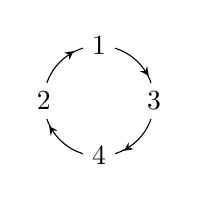
\begin{tikzpicture}
		[decoration = {markings,
			mark = between positions 0.1 and 1 step 0.25 with
			{\arrow[>=stealth]{<}}}]
		\draw[postaction = decorate] (0, 0) circle [radius = 0.7 cm];
		\path	(90 :0.7 cm) node[fill=white]{$1$}
				(180:0.7 cm) node[fill=white]{$2$}
				(270:0.7 cm) node[fill=white]{$4$}
				(360:0.7 cm) node[fill=white]{$3$} ;
	\end{tikzpicture}
\end{center}
	
\end{definition}

\begin{definition}[\textbf{Composition of $\sigma$ and $\tau$}]
	\begin{description}
		\item $\sigma \circ \tau(i) = \sigma(\tau(i))$
		\item $\sigma \circ \tau(1) = \sigma(3) = 3$
		\item $\sigma \circ \tau(2) = \sigma(1) = 2$ 
		\item $\sigma \circ \tau(3) = \sigma(4) = 1$
		\item $\sigma \circ \tau(4) = \sigma(2) = 4$
	\end{description}
	still a bijection! $\sigma \circ \tau$ is a bijection. 

	Expression $\sigma \circ \tau : $ 
	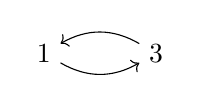
\begin{tikzpicture}[node distance = 1cm] 
		\node (1) {$1$};
		\node (2) [right=of 1] {$3$};
		\draw[->] (1) to [bend right] (2);
		\draw[->] (2) to [bend right] (1);
	\end{tikzpicture}
	$\overset{2}{\circlearrowright}
	\overset{4}{\circlearrowright}$
\end{definition}

\begin{notation}[\textbf{"cycles"}]
	\begin{align*}
		\sigma =& (1 2 4)(3) = (2 4 1)(3) \\
		%
		\tau =& (1 3 4 2)\\
		%
		\sigma \circ \tau =& (1 3)(2)(4)
	\end{align*}
\end{notation}

\begin{definition}
	$S_n$ is the set of all permutations of $\{1, \cdots, n\}$. 
\end{definition}

\begin{definition}
	Given $r \in S_n$, $A, B \in M_n(\mF)$, we write
	$A \overset{R:\sigma}{\longrightarrow} B$ to mean that $B$ is obtained from
	$A$ by moving 
	\[
		\Row_i(A) + \Row_{\sigma} (i)(B), \qquad \text{for } 0 \leq i \leq n
	\]
\end{definition}

{\color{Brown}
	\textbf{Example: }
	$\sigma = (1 2 4)$
	\[
		A = 
		\begin{pmatrix}
			-- & r_1 & -- \\
			-- & r_2 & -- \\
			== & r_3 & -- \\
			-- & r_4 & -- 
		\end{pmatrix}
		\overset{R: \sigma}{\longrightarrow} 
		\begin{pmatrix}
			-- & r_4 & -- \\
			-- & r_1 & -- \\
			== & r_3 & -- \\
			-- & r_2 & -- 
		\end{pmatrix}
		=B
	\]
	$\sigma(a)=1$ $a = \sigma^{-1}(1)$

	$B$ can also be written as 
	\[
		\begin{pmatrix}
			-- & r_{\sigma^{-1}}(1) & -- \\
			-- & r_{\sigma^{-1}}(2) & -- \\
			== & r_{\sigma^{-1}}(3) & -- \\
			-- & r_{\sigma^{-1}}(4) & -- 
		\end{pmatrix}
	\]
}

\begin{definition}
	Given $\sigma \in S_n$, the permutation matrix associated to $\sigma$ is 
	the matrix $P_{\sigma}$ which is obtained from $I_n$ by 
	$\overset{R:\sigma}{\longrightarrow}$.
	\[
		I_n \overset{R:\sigma}{\longrightarrow} P_{\sigma}
	\]
	\[
		I_n = 
		\begin{pmatrix}
			e_1 \\
			e_2 \\
			\vdots \\
			e_n
		\end{pmatrix}
		\overset{R:\sigma}{\longrightarrow} P_{\sigma}
		=
		\begin{pmatrix}
			-- & e_{\sigma^{-1}}(1) & -- \\
			-- & e_{\sigma^{-1}}(2) & -- \\
			   & \vdots & \\
			-- & e_{\sigma^{-1}}(n) & -- 
		\end{pmatrix}
	\]
\end{definition}

{\color{Brown}
	\textbf{Recall: }$\sigma = (1 2 4)(3)$

	\begin{align*}
		P_{\sigma} =& 
		\begin{pmatrix}
			-- & e_{\sigma^{-1}}(1) & --	\\
			-- & e_{\sigma^{-1}}(2) & --	\\
			== & e_{\sigma^{-1}}(3) & --	\\
			-- & e_{\sigma^{-1}}(4) & -- 
		\end{pmatrix}
		= 
		\begin{pmatrix}
			-- & e_4 & --	\\
			-- & e_1 & --	\\
			== & e_3 & --	\\
			-- & e_2 & --
		\end{pmatrix}
		= 
		\begin{pmatrix}
			0 & 0 & 0 & 1	\\
			1 & 0 & 0 & 0	\\
			0 & 0 & 0 & 1	\\
			0 & 1 & 0 & 0
		\end{pmatrix}\\
		= &
		\begin{pmatrix}
			| & | & | & |	\\
			e_2 & e_4 & e_3 & e_1	\\
			| & | & | & |	\\
		\end{pmatrix}
		= 
		\begin{pmatrix}
			| & | & | & |	\\
			e_{\sigma(1)} & e_{\sigma(2)} & e_{\sigma(3)} & e_{\sigma(4)}	\\
			| & | & | & |	\\
		\end{pmatrix}
	\end{align*}
}
\begin{description}
	\item $P_{\sigma}$ is a very special matrix
	\item Each row and column has exactly one "1"
	\item For this matrix $\Row_i(P_{\sigma}) = e_{\sigma^{-1}}(i)$
		and $\Col_i(P_{\sigma}) = e_{\sigma}(i)$
	\item $P_{\sigma^{-1}} = (P_{\sigma})^t$
	\item $P_{\sigma} e_j = e_{\sigma}(j)$
\end{description}

\begin{theorem}
	$\sigma \in S_n$, $A \in M_{n\times n} (\mF)$
	\begin{enumerate}
		\item $P_{\sigma} A$ is the result of applying $\sigma$ to the rows of 
			$A : A \overset{R: \sigma}{\longrightarrow} P_{\sigma}A$
		\item $A P_{\sigma}$ is the result of applying $\sigma$ to the column
			of $A:A \overset{C: \sigma}{\longrightarrow} AP_{\sigma}$
	\end{enumerate}
\end{theorem}
\begin{proof}
	(2) Suppose $(\sigma^{-1})^{-1} = \tau$ (bijection), 
	$(\sigma^{-1}) = (\tau^{-1}) \rightarrow \sigma = \tau$, 
	$1 \overset{\sigma}{\longrightarrow}i 
	\overset{\sigma^{-1}}{\longrightarrow} 1$. 

	\begin{align*}
		A = &
		\begin{pmatrix}
			| & | &  & |	\\
			C_1 & C_2 & \cdots & C_n	\\
			| & | &  & |	\\
		\end{pmatrix}
		\overset{\sigma^{-1}}{\longrightarrow}
		\begin{pmatrix}
			| & | &  & |	\\
			C_{(\sigma^{-1})^{-1}}(1) & C_{(\sigma^{-1})^{-1}}(2) &
			\cdots & C_{(\sigma^{-1})^{-1}}(n)	\\
			| & | &  & |	\\
		\end{pmatrix}\\
		=&
		\begin{pmatrix}
			| & | &  & |	\\
			C_{\sigma}(1) & C_{\sigma}(2) &
			\cdots &C_{\sigma}(n)	\\
			| & | &  & |	\\
		\end{pmatrix}
		= B
	\end{align*}
	We want $B = A P_{\sigma}$, 
	$\Col_j(AP_{\sigma}) = A\cdots \Col_j(P_{\sigma}) = A \cdot e_{\sigma}(j)
	= A_{\sigma}(j)$ 

	$\Col_j(B) = \Col_j$. 
\end{proof}

\begin{corollary}
	$P_{\sigma} P_{\tau} = P_{\sigma \tau}$
\end{corollary}
\begin{proof}
	\[
		I_n \overset{R:\sigma \tau} {\longrightarrow} P_{\sigma \tau}
		= 
		\begin{pmatrix}
			-- & r_{\sigma \tau^{-1}}(1) & --\\
			-- & r_{\sigma \tau^{-1}}(2) & --\\
			   & \vdots & \\
			-- & r_{\sigma \tau^{-1}}(n) & --\\
		\end{pmatrix}
	\]
	
	\[
		I_n \overset{R:\tau} {\longrightarrow} P_{\tau}
		= 
		\begin{pmatrix}
			-- & r_{\tau^{-1}}(1) & --\\
			-- & r_{\tau^{-1}}(2) & --\\
			   & \vdots & \\
			-- & r_{\tau^{-1}}(n) & --\\
		\end{pmatrix}
		\overset{R:\sigma} {\longrightarrow}
		\begin{pmatrix}
			-- & r_{\sigma^{-1} \tau^{-1}}(1) & --\\
			-- & r_{\sigma^{-1}\tau^{-1}}(2) & --\\
			   & \vdots & \\
			-- & r_{\sigma^{-1}\tau^{-1}}(n) & --\\
		\end{pmatrix}
	\]
	$(\sigma \tau)^{-1} = \sigma^{-1} \tau^{-1}$
\end{proof}



%------------------------------------------------------------------------------
%------------------------------------------------------------------------------
%------------------------------------------------------------------------------
%------------------------------------------------------------------------------
%------------------------------------------------------------------------------
%------------------------------------------------------------------------------
%------------------------------------------------------------------------------
	\newpage
	\subsection{Feb 26}

	\begin{definition}
		If $A, B$ matrices of some size, write $A \leadsto B$ to mean we can
		obtain $B$ from $A$ by some sequence of elements row and/or solumn 
		operations. 
	\end{definition}

	{\color{Brown}
	\textbf{Example: } $\mF= \mR$
	\[
		A = 
		\begin{pmatrix}
			2	& 4	& 1 & 0\\
			-1	& -2& 1 & 3\\
			3 & 6 & 0 & -3 
		\end{pmatrix}
		\begin{pmatrix}
			1 & 0 & 0 & 0\\
			0 & 1 & 0 & 0\\
			0 & 0 & 0 & 0
		\end{pmatrix}
	\]
	
	\[
		A \overset{R_1 \rightleftarrows R_2}{\longrightarrow}
		\begin{pmatrix}
			-1 & -2 & 1 & 3\\
			2 & 4 & 1 & 0\\
			3 & 6 & 0 & -3
		\end{pmatrix}
		\overset{R_2 \leftarrow R_2+2R_1} {\longrightarrow}
		\begin{pmatrix}
			-1 & -2 & 1 & 3\\
			0 & 0 & 3 & 6\\
			3 & 6 & 0 & -3
		\end{pmatrix}
	\]
	\[
		\overset{R_3 \leftarrow R_3 + 3R}{\longrightarrow}
		\begin{pmatrix}
			-1 & -2 & 1 & 3\\
			0 & 0 & 3 & 6 \\
			0 & 0 & 3 & 6 
		\end{pmatrix}
		\overset{C_1 \leftarrow (-1)C_1}{\longrightarrow}
		\begin{pmatrix}
			1 & -2 & 1 & 3\\
			0 & 0 & 3 & 6\\
			0 & 0 & 3 & 6
		\end{pmatrix}
		\overset{C_2 \rightleftarrows C_3}{\longrightarrow}
		\begin{pmatrix}
			1 & 1 & -2 & 3\\
			0 & 3 & 0 & 6\\
			0 & 3 & 0 & 6
		\end{pmatrix}
	\]
	\[
		\overset{R_3 \leftarrow R_3 + (-1)R_2}{\longrightarrow}
		\begin{pmatrix}
			1 & 1 & -2 & 3\\
			0 & 3 & 0 & 6 \\
			0 & 0 & 0 & 0
		\end{pmatrix}
		\overset{R_2 \leftarrow \frac 13 R_2}{\longrightarrow}
		\begin{pmatrix}
			1 & 1 & -2 & 3\\
			0 & 1 & 0 & 2\\
			0 & 0 & 0 & 0
		\end{pmatrix}
	\]
	\[
		\overset{C_3 \leftarrow C_3 + 2C_1}{\longrightarrow}
		\begin{pmatrix}
			1 & 1 & 0 & 3\\
			0 & 1 & 0 & 2\\
			0 & 0 & 0 & 0
		\end{pmatrix}
		\overset{C_4 \leftarrow C_4 + (-2)C_1}{\longrightarrow}
		\begin{pmatrix}
			1 & 1 & 0 & 1\\
			0 & 1 & 0 & 0\\
			0 & 0 & 0 & 0
		\end{pmatrix}
	\]
	\[
		\overset{R_1 \leftarrow R_1 + (-1)R_2}{\longrightarrow}
		\begin{pmatrix}
			1 & 0 & 0 & 1\\
			0 & 1 & 0 & 0\\
			0 & 0 & 0 & 0
		\end{pmatrix}
		\overset{C_1 \leftarrow C_1 + (-1)C_1}{\longrightarrow}
		\begin{pmatrix}
			1 & 0 & 0 & 0\\
			0 & 1 & 0 & 0\\
			0 & 0 & 0 & 0
		\end{pmatrix}
	\]
	For $i = 1, \cdots,, 11$, let $E_i$ be the elementary corresponding to step
	i, 
	\[
		E_1 =
		\begin{pmatrix}
			0 & 1 & 0\\
			1 & 0 & 0\\
			0 & 0 & 1
		\end{pmatrix}
	\]
	\[
		E_4 = 
		\begin{pmatrix}
			1 & 0 & 0 & 0	\\
			0 & 1 & 0 & 0	\\
			0 & 0 & 1 & 0	\\
			0 & 0 & 0 & 1	\\
		\end{pmatrix}
	\]
	$\underbrace{E_{10} E_7 E_6 E_3 E_2E_1}_{P} A 
	\underbrace{E_4 E_5E_8 E_9E_{11}}_{Q} = D$.
	$P$ and $Q$ are invertible.\\
	}


	\begin{theorem}
		Suppose $A, B \in M_{m\times n}(\mF)$, if $A \leadsto B$ then $\exists$
		invertible $P \in M_{m\times m} (\mF)$ and invertible 
		$Q \in M_{n \times n} (\mF)$ s.t. $PAQ = B$. 
	\end{theorem}
	\begin{proof}
		Pick a sequence of elementary row/col operations taking $A$ to $B$.
		Let $Q_1, Q_k$ be the row operations in this sequence, $Q_1', \cdots, 
		Q_2'$ be the column operations. 

		Let $E_i$ be the elementary matrix corresponding to $Q_i$.
		$I_m \overset{Q_i}{\longrightarrow} E_i$. 

		Let $E_j$ be the elementary matrix corresponding to $Q_j'$. 

		$P = E_k \cdots, E_2E_1$\\
		$Q = E_1' E_2' \cdots E_e'$

		Then $PAQ = B$. 
	\end{proof}

	\begin{theorem}
		$\forall A \in M_{m\times n} (\mF)$, $\exists D \in M_{m\times n}(\mF)$
		of the form
		\[
			D = 
			\begin{pmatrix}
				I_r & \rvline & O_{r \times (n-r)} \\ \hline
				O_{(m-r)\times r} & \rvline & O _{(m-r)\times(n-r)} 
			\end{pmatrix}
			\qquad (\text{for some } r\geq 0)
		\]
		s.t. $A \leadsto D$. 
	\end{theorem}
	\begin{proof}
		If $A = O_{m\times n}$, done. Else, $A$ has a nonzero entry somewhere,
		use Type (1) operations, can move this entry to $(1, 1)$ position,
		making this entry = 1, with a type (2) operations, apply type 3 
		operations to get  
		\[
			\leadsto 
			\begin{pmatrix}
				1 & \rvline & 0 & 0 & \cdots & 0\\ \hline
				0 & \rvline \\
				0 & \rvline \\
				\vdots & \rvline\\
				0 & \rvline\\
			\end{pmatrix}
		\]
		
	\end{proof}

	\begin{corollary}
		$\forall A$, $\exists$ invertible $P, Q$ s.t. 
		\[
			PAQ =
			\begin{pmatrix}
				I_r & O \\
				O & O
			\end{pmatrix}
		\]
	\end{corollary}
	\begin{proof}
		Find $P$ and $Q$, 
		\begin{enumerate}
			\item find $E_1, \cdots, E_k, E_1', \cdots, E_e'$ multiply...
		\end{enumerate}
	\end{proof}

%------------------------------------------------------------------------------
%------------------------------------------------------------------------------
%------------------------------------------------------------------------------
%------------------------------------------------------------------------------
%------------------------------------------------------------------------------
%------------------------------------------------------------------------------
%------------------------------------------------------------------------------
\newpage
\subsection{Feb 28}
\begin{corollary}
	If $A \leadsto B$, then
	\begin{enumerate}
		\item $B \leadsto A$ 
		\item $A^t \leadsto B^t$
	\end{enumerate}
\end{corollary}
\begin{proof}
	\begin{enumerate}
		\item Row and Column operations are reversible
		\item Change row operations to column operations and vice versa
	\end{enumerate}
\end{proof}

\begin{definition}
	Let $A$ be an $m \times n$ matrix over $\mF$. 
	\begin{enumerate}
		\item The row space of $A$ is the span in $\mF^n$, of the rows of $A$. 
		\[
			A = 
			\begin{pmatrix}
				a_{11} & \cdots & a_{1n}	\\
				\vdots & \cdots & \vdots	\\
				a_{m1} & \cdots & a_{mn}	
			\end{pmatrix}
		\]
		\item The column space of $A$ is the span in $\mF^n$ of the columns of
			$A$. 

			\textbf{Recall:} $L_A : \mF^n \to \mF^n$ $R(L_A) =$ the column 
			space of $A$ 

		\item The null space of $A$, denoted $N(A)$ is 
			$N(L_A) = \{x \in \mF^n: Ax = 0\}$, a subsapce $\mF^n$

			\textbf{Recall:} 
			$\underbrace{\dim(\text{column space of } A)}_{rank(L_A)}
			+ \underbrace{\dim(N(A))}_{nullity(L_A)} = \dim \mF^n = n$.  
	\end{enumerate}
\end{definition}

\begin{definition}
	\begin{description}
		\item \textbf{rank of $A$} is $\rank(L_A)$
		\item \textbf{nullity of $A$} is $\nullity(L_A)$
	\end{description}
\end{definition}

\begin{theorem}
	If $A \in M_{m\times n} (\mF)$ and $Q \in M_{m\times n}(\mF)$, with $Q$
	invertible, then $R(L_AQ) = R(L_A)$. 
\end{theorem}
\begin{proof}
	$AQ$ is $m\times n$, $L_{AQ}:$
	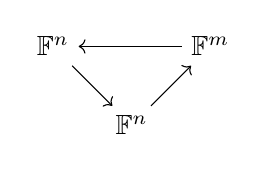
\begin{tikzpicture}
			\node[fill=white] (A) at (2, 1) {$\mF^n$}; 
			\node[fill=white] (B) at (4, 1) {$\mF^m$}; 
			\node[fill=white] (C) at (3, 0) {$\mF^n$}; 
			\draw[->] (B) -- (A) ;
			\draw[->] (C) -- (B);
			\draw[->] (A) -- (C);
		\end{tikzpicture}

	$L_{AQ} = L_A\circ L_Q$, $L_Q$ is an isomorphism hence is surjective. 
	\begin{align*}
		R(L_{AQ}) =& \{L_{AQ}: x\in \mF^n\} \\
		=& \{L_A(L_Q(x)): x\in \mF^n\} \\
		=& \{L_A(y): y\in\mF\} \tag{as $L_Q$ is surjective} \\
		=& R(L_A) 
	 \end{align*}
\end{proof}

\begin{corollary}
	IF $A \leadsto B$ , entirely by column operations, then $A$ and $B$ have 
	the same column space.
\end{corollary}
\begin{proof}
	$A \leadsto B$ by column operations $\Rightarrow B = AQ$, for some 
	invertible $Q$.
	
	Then, 
	\begin{align*}
		\ColSpace \ of \ B 
		=& \ColSpace \ of \ AQ		\\
		=& R(L_{AQ})	\\
		=& R(L_A) \tag{Thm 1}	\\
		=& \ColSpace \ of \ A
	\end{align*}
\end{proof}

\begin{corollary}
	IF $A \leadsto B$ , entirely by row operations, then $A$ and $B$ have 
	the same row space.
\end{corollary}
\begin{proof}
	$A \leadsto B$ by row operations

	$\Rightarrow A^t \leadsto B^t$ by column operations

	$\Rightarrow A^t, B^t$ have same column space

	$\Rightarrow A, B$ have same row space
\end{proof}

\begin{lemma}
	Suppose $V$ is finite dimensional, $T:V\cong V'$, and $W$ is a subspace of
	$V$. 

	Let $W' = \{T(w) : w \in W\}$, a subspace of $V'$, then $\dim(W) = \dim(W')$.
\end{lemma}
\begin{proof}
	Let $B_w$ be a basis for $W = \{w_1, \ldots, w_k\}$. 

	\textbf{Claim:} $\{T(w_1), \ldots, T(w_k)\}$ is a basis for $W$. 
	\begin{alignat*}{2}
		& & a_1T(w_1) + \ldots + a_kT(w_k) =& 0\\
		\Rightarrow &\qquad & T(a_1w_1 + \ldots + a_kw_k) =& 0\\
		\Rightarrow &\qquad & a_1w_1 + \ldots + a_kw_k \in N(T) =& \{0\} \\
		\Rightarrow &\qquad & a_1w_1 + \ldots + a_kw_k =& 0\\
		\Rightarrow &\qquad & a_1 = \ldots = a_k =& 0
	\end{alignat*}
\end{proof}

\begin{theorem}
	Suppose $A \in M_{m\times n} (\mF)$. $P\in M_{m\times m}(\mF)$, $P$ 
	invertible. Then $\dim(\ColSpace \ of \ A) = \dim(\ColSpace \ of \ PA)$. 
	i.e. $\rank(A) = \rank(PA)$. 
\end{theorem}
\begin{proof}
	$L_{PA} : \mF^n \to \mF^m$,

	Let $W = R(L_A)$, let $W' = \{L_P(y): y \in W\}$. 

	We know $\dim(W) = \dim(W')$. (lemma)
	
	\textbf{Note:} 
	\begin{align*}
		W' =& \{L_P(y) : y \in W\}	\\
		=& \{L_P(L_A(x)): x \in \mF^n\}	\\
		=& \{L_{PA}(x): x \in \mF^n\}	\\
		=& R(L_{PA}) 
	\end{align*}
	So $\dim(\ColSpace \ of \ A) = \dim(R(L_A)) = \dim(R(L_{PA}))
	= \dim(\ColSpace \ of \ PA)$. 
\end{proof}


\begin{corollary}
	IF $A \leadsto B$ entirely by row operations then $\rank(A) = \rank(B)$. 
\end{corollary}
\begin{proof}
	$A \leadsto B$ by row operations, $\Rightarrow B = PA$ for some invertible
	$P$ $\Rightarrow \rank(A) = \rank(PA) = \rank(B)$. 
\end{proof}

\begin{corollary}
	If $A \leadsto B$ then $\rank(A) = \rank(B)$. 
\end{corollary}
\begin{proof}
	If $A \leadsto B$, then $B = PAQ$ then $\rank(A) = \rank(PA) = \rank(PAQ)$.
\end{proof}

\begin{corollary}
	If $A \leadsto \begin{pmatrix} I_r & 0 \\ 0 & 0
	\end{pmatrix}$ then $\rank(A) = r$. 
\end{corollary}


\begin{corollary}
	For any $A$, $\rank(A) = \rank(A^t)$. i.e. $\ColSpace$ of $A$ and row
	space of $A$ have same dimension. 
\end{corollary}
\begin{proof}
	\[
		A \leadsto 
		\begin{pmatrix}
			I_r & \rvline & 0 \\ \hline
			0 & \rvline & 0
		\end{pmatrix}
		\qquad r = \rank A
	\]
	\[
		A^t \leadsto 
		\begin{pmatrix}
			I_r^t & \rvline & 0 \\ \hline
			0 & \rvline & 0
		\end{pmatrix}
		\qquad r = \rank A^t
	\]
\end{proof}







%------------------------------------------------------------------------------
%------------------------------------------------------------------------------
%------------------------------------------------------------------------------
%------------------------------------------------------------------------------
%------------------------------------------------------------------------------
%------------------------------------------------------------------------------
%------------------------------------------------------------------------------
%------------------------------------------------------------------------------
\newpage
\subsection{March 2}


Suppose $A \in M_{}(\mF)$, $A$ can be transformed: 
\[
	A^t \leadsto 
	\begin{pmatrix}
		I_r^t & \rvline & 0 \\ \hline
		0 & \rvline & 0
	\end{pmatrix}
	\qquad r = \rank A^t
\]
$r = \rank(A)$. 

\begin{theorem}[\textbf{Invertible Matrix Theorem}]
	For $A \in M_{n\times n}(\mF)$, TFAE
	\begin{enumerate}
		\item $A$ is invertible
		\item $\rank(A) = n$
		\item A can be written as a product of elementary matrices. 
		\item $A \leadsto I_n$
		\item $A \leadsto I_n$ by row operations
	\end{enumerate}
\end{theorem}
\begin{proof}
	From $5$ to $1$, 

	$I_n = E_k\cdots E_1A$ 

	\[
		I_n = EA \Rightarrow AE = I_n
	\]
	So $A$ is invertible, and $A^{-1} = E$. Hence, $E$ is invertible. 

	$\Rightarrow E^{-1} I_n = E^{-1}(EA) \Rightarrow E^{-1} = A$. 

	$E^{-1} = (E_k \cdots E_1)^{-1}$. 

	\[
		E^{-1} = (E_k\cdots E_1)^{-1} = E^{-1} \cdots E^{-1}
	\]
	and each $^{-1}$ is an elementary operation, hence proves 3. 

	If $A \leadsto I_n = 
	\begin{pmatrix}
		I_n & \rvline& \cdots \\ \hline
		\cdots &\rvline &\cdots \\
	\end{pmatrix}
	$.

	$1$ 
	$\Rightarrow L_A$ is an isomorphism.

	$\Rightarrow L_A$ is surjective.  
	
	$\Rightarrow R(L_A) = \mF^n$ 

	$\Rightarrow \dim(R(L_A)) = n \Rightarrow \rank(A) = n$. 

	$4$ to $1$, $3$, Assume (4), then $I_n = PAQ$, 
	$\Rightarrow P^{-1}I_nQ^{-1} = P^{-1}(PAQ)Q^{-1}$,

	$\Rightarrow P^{-1}Q^{-1} = A$ so $A$ is invertible. 

	$4$ to $5$, 
	$A \leadsto I_n \Rightarrow I_n = (PA)Q$, $P, Q$ invertible. 

	$QI_nQ^{-1} = Q(PAQ)Q^{-1}$. 

	$I_n = QPA \Rightarrow A \leadsto I_n$ by row operations. 

\end{proof}

Suppose $A \leadsto I_n$ by row operations, then $I_n = E_k \cdots E_2 E_1 A$


$\Rightarrow I_n A^{-1} = E_k \cdots E_2 E_1 A A^{-1}$ 

$\Rightarrow A^{-1} = E_k \cdots E_2 E_1 I_n$. 

Show: exactly the same sequence of row operations, transforming $A \leadsto I_n$
also transforms $I_n \leadsto A^{-1}$. 


\begin{algorithm}
	To find $A^{-1}$ (when it exists) 
	\begin{enumerate}
		\item Form $n \times 2n$ matrix $A I_n$ 
		\item Apply row operations transform to $(I_n  \blacksquare)$ 
			$\blacksquare$: will be $A^{-1}$.  \\
	\end{enumerate}
\end{algorithm}

{\color{Brown}
\textbf{Example: }
\[
	A = 
	\begin{pmatrix}
		1 & -3 & 1\\
		1 & 0 & 2\\
		0 & 1 & 0 
	\end{pmatrix}
\]

\[
	\begin{pmatrix}
		1 & -3 & 1 & \rvline & 1 & 0 & 0\\
		1 & 0 & 2 & \rvline & 0 & 1 & 0	\\
		0 & 1 & 0 & \rvline & 0 & 0 & 1	\\
	\end{pmatrix}
	\overset{R_1 \la R_1 + 3R_3}{\longrightarrow}
	\begin{pmatrix}
		1 & 0 & 1 & \rvline & 1 & 0 & 3 \\
		1 & 0 & 2 & \rvline & 0 & 1 & 0	\\
		0 & 1 & 0 & \rvline & 0 & 0 & 1	\\
	\end{pmatrix}
	\overset{R_2 \la R_2 - R_1}{\longrightarrow}
	\begin{pmatrix}
		1 & 0 & 1 & \rvline & 1 & 0 & 3		\\
		0 & 0 & 1 & \rvline & -1 & 1 & -3	\\
		0 & 1 & 0 & \rvline & 0 & 0 & 1		\\
	\end{pmatrix}
\]

\[
	\overset{R_2 \leftrightarrows R_3}{\longrightarrow}
	\begin{pmatrix}
		1 & 0 & 1 & \rvline & 1 & 0 & 3\\
		0 & 1 & 0 & \rvline & 0 & 0& 1	\\
		0 & 1 & 0 & \rvline & 0 & 0 & 1	\\
	\end{pmatrix}
	\overset{R_1 \la R_1 - R_3}{\longrightarrow}
	\begin{pmatrix}
		1 & 0 & 0 & \rvline & 2 & -1 & 6\\
		0 & 1 & 0 & \rvline & 0 & 0 & 1	\\
		0 & 0 & 1 & \rvline & -1 & 1 & -3	\\
	\end{pmatrix}
\]

$\Rightarrow A^{-1} = 
\begin{pmatrix}
	2 & -1 & 6	\\
	0 & 0 & 1	\\
	-1 & 1 & -3	\\
\end{pmatrix}$

}

%------------------------------------------------------------------------------
%------------------------------------------------------------------------------
%------------------------------------------------------------------------------
%------------------------------------------------------------------------------
%------------------------------------------------------------------------------
%------------------------------------------------------------------------------
%------------------------------------------------------------------------------
%------------------------------------------------------------------------------

\newpage
\subsection{March 4}
Consier a system of $m$ linear equations in $n$ variables. 

\[
	S 
	\begin{cases}
		a_{11} x_1 + a_{12} x_1 + \cdots + a_{1n}x_n = b_1\\
		a_{21} x_1 + a_{22} x_1 + \cdots + a_{2n}x_n = b_1\\
		\vdots	\\
		a_{n1} x_1 + a_{n2} x_1 + \cdots + a_{nn}x_n = b_1\\
	\end{cases}
\]
$a_{ij}, b_i \in$ some field $\mF$. 

Then we want solutions $x = (x_1, \cdots, x_n) \in \mF^n$. 

Can write $(S)$ as 
\[
	\begin{pmatrix}
		a_{11} & a_{12} & \cdots & a_{1n}	\\
		\vdots &	\\
		a_{m1} & a_{m2} & \cdots & a_{mn}
	\end{pmatrix}
	\begin{pmatrix}
		x_1	\\
		x_2	\\
		\vdots	\\
		x_n
	\end{pmatrix}
	=
	\begin{pmatrix}
		b_1	\\
		\vdots	\\
		b_m
	\end{pmatrix}
\]
or compactly as $AX = b$. 

A is the coefficient matrix of (S). 

$A \in M_{m\times n}(\mF)$, $b \in \mF^m$, the RHS vector.

\[
	X = 
	\begin{pmatrix}
		x_1		\\
		\vdots	\\
		x_n
	\end{pmatrix}
\]
is a vector of formal variables. 

Solutions: vectors $x = \begin{pmatrix}x_1 \\ \vdots \\ x_n \end{pmatrix} \in
\mF^n$, such that $Ax = b$. 

(S) is homogenous if $b = 0$ else, (S) is nonhomogeneous. 

If $b\neq 0$, then the system $AX = 0$ is the homogeneous system associated to
$AX = b$. 

The solution set to $AX = b$ is $\{x \in \mF^n : Ax = b\} =: Sol(AX=b)$. \\

\begin{definition}
	$AX = b$ is consistent if $Sol(AX=b) \neq \varnothing$, else $AX=b$ is 
	inconsistent. \\
\end{definition}

\begin{theorem}
	Let $A \in M_{m\times n} (\mF)$, $b\in \mF^m$, consider the system $AX=b$,

	\begin{enumerate}
		\item If $b = 0$, then $Sol(AX = 0) = N(A)$.
		\item $AX = b$ is consistent $\Leftrightarrow b \in$ column space of 
			$A$ $(=R(L_A))$. 
		\item If $AX = b$ is consistent, then $Sol(AX=b)$ is a translation
			of $N(A)$, i.e. $Sol(AX=b) = u + N(A)$, where u can be any solution
			to $AX=b$. 
	\end{enumerate}
\end{theorem}
\begin{proof}
	(1) For $x \in \mF^n$,
	\begin{alignat*}{2}
		& & & x \in Sol(AX = 0) \\
		\Leftrightarrow & \qquad & &Ax = 0 \\
		\Leftrightarrow & \qquad & &L_A(x) = 0 \\
		\Leftrightarrow & \qquad & &x \in N(L_A) = N(A)
	\end{alignat*}
	
	(2) $AX = b$ is consistent 
	\begin{alignat*}{2}
		& & &AX = b \ \text{is consistent}	\\
		\Leftrightarrow & \qquad & & Sol(AX = b) \neq \varnothing	\\
		\Leftrightarrow & \qquad & & \exists x \in \mF^n. Ax = b	\\
		\Leftrightarrow & \qquad & & \exists x \in \mF^b, L_A(x) = b	\\
		\Leftrightarrow & \qquad & & b \in R(L_A) = \ColSpace \ of \ A	
	\end{alignat*}
	
	(3) Assume $AX = b$ is consistent, pick a solution, say $u \in \mF^n$, 
	(So $Au = b$). 

	I'll prove that $Sol(AX = b) \subseteq u + N(A)$. 
	So $Ax = b = Au$, so $A(x-u) = Ax - Au = 0$. 

	$\Rightarrow x - u \in N(A)$
	
	$\Rightarrow x = u + (X - u) \Rightarrow x \in u + N(A)$. 

	$u + N(A)\subseteq Sol(AX = b)$, suppose $x \in u + N(A)$, 

	\begin{alignat*}{2}
		\Rightarrow & \qquad & x =& u + v	\\
		\Rightarrow & \qquad & Ax =& A(u+v)	\\
					& &		=& Au + Av	\\
					& &		=& b + 0 = b	\\
		\Rightarrow & \qquad & x \in& Sol(AX=b). \\
	\end{alignat*}
\end{proof}


\textbf{Goal:} Given $AX = b$, 
\begin{enumerate}
	\item Determine whether $AX = b$ is consistent
	\item If it is, then find one solution $u$ and find basis 
		$\{x_1, \cdots, x_k\}$ for $N(A)$.
		Then $Sol(AX = b) = u + \Span(\{x_1, \cdots, x_k\}) = \{u + c_1x_1 +
		\cdots + c_kx_k, c_1\cdots c_k \in \mF\}$. \\
\end{enumerate}

\begin{definition}
	Suppose $A \in M_{m\times n}(\mF)$, $b \in \mF^m$, the $m\times(n+1)$
	matrix $(A|b)$ is the \textbf{augmented matrix} of $AX = b$. \\
\end{definition}

\begin{lemma}
	Given $A \in M_{m\times n} (\mF)$, $b \in \mF^m$, if $(A|b) \leadsto
	(A'|b')$ using only row operations, then 
	\[
		Sol(AX = b) = Sol(A'X = b')
	\]
\end{lemma}
\begin{proof}
	Suppose $(A|b)\leadsto (A'|b')$ via row operations, 
	
	so $\exists$ invertible $P \in M_{m\times m}(\mF)$ s.t. $P(A|b) = (A'|b')$. 
	$\Rightarrow PA = A' \qquad and \qquad Pb = b'$
	and $A = P^{-1}A'$ and $b = P^{-1}b'$. 

	\textbf{Claim: }
	\[
		Sol(AX = b) \subseteq Sol(A'X = b')
	\]
	Let $x \in Sol(AX = b)$, i.e. $Ax = b$,

	$\Rightarrow (PA)x = Pb$ 

	$\Rightarrow A'x = b'$. 

	i.e. $x \in Sol(A'X = b')$. 
\end{proof}

\begin{definition}
	A matrix is in \textbf{Reduced Row Echelon Form} (RREF) if all of the 
	following hold: 
	\begin{enumerate}
		\item If a row has a nonzero entry, the 1st such = 1. (called 
			the \textbf{leading one} of the row)
		\item If a column contains a leading one, all other entries
			in that column = 0. 
		\item Lower (nonzero) columns have leadings further to right. 
		\item All zero rows \underline{of any} are at bottom
	\end{enumerate}
\end{definition}

{\color{Brown}
\textbf{Non-Examples of RREF: }
\[
	\begin{pmatrix}
		0 & 1 & 0 & 2	\\
		0 & 0 & 0 & 1	\\
		0 & 0 & 0 & 0
	\end{pmatrix}
\]
\textbf{Example: }
\[
	\begin{pmatrix}
		0 & 1 & 0 & 2	\\
		0 & 0 & 0 & 1	\\
		0 & 0 & 0 & 0
	\end{pmatrix}
\]


}






%------------------------------------------------------------------------------
%------------------------------------------------------------------------------
%------------------------------------------------------------------------------
%------------------------------------------------------------------------------
%------------------------------------------------------------------------------
%------------------------------------------------------------------------------
%------------------------------------------------------------------------------
%------------------------------------------------------------------------------
\newpage
\subsection{RREF and Solving Linear Equations - March 6}
\begin{theorem}
	Every $A \in M_{m\times n}(\mF)$ can be converted to a matrix in RREF,
	by a sequence of elementary row operations. 
\end{theorem}
\begin{proof}
	If $A = O_{m\times n}$, done. 

	Else, pick first column, say $\Col_j(A)$, which is nonzero, using row 
	operations, move nonzero entry in column $j$, to position $(1, j,)$, change
	it to $1$, clear all other entries in $\Col j$, 

	get 
	\[
		\leadsto A' = 
		\begin{pmatrix}
			0 & \cdots & 0	& 1		& \rvline	& *	& \cdots & *	\\	\hline
			0 & \cdots & 0	& 0		& \rvline	&  	&  & 	\\
			  &		   &	& \vdots& \rvline	&	&   B    &		\\
			0 & \cdots & 0	& 0		& \rvline	& 	&   & 	\\
		\end{pmatrix}
	\]
	Next, if $B = O_{(m-1)\times (n-j)}$, we are done, else
	find $1st$ column of $A$, say $\Col_j(A)$, which meets a nonzero entry of 
	$B$, pick a nonzero entry of $B$ in that column, move it to position 
	$(2, j_2)$, change it to $1$, clear all other entries in that column. 
	\[
		\leadsto A'' = 
		\begin{pmatrix}
			0 & \cdots  & 1 & * & \cdots & * & 0 & * & \cdots & * \\ \hline
			0 & \cdots  & 0 & * & \cdots & 0 & 1 & * & \cdots & * \\ \hline
			0 & \cdots  & 0 & 0 & \cdots & 0 & 0 & 	&  	& 	\\
			  &		    &   &   &	    &   &	&   &	&	\\
			0 & \cdots  & 0 & 0 & \cdots & 0 & 0 &   & 	&	\\
		\end{pmatrix}
	\]
	Eventually stops, resulting matrix is in RREF.
\end{proof}

\begin{proposition}
	If $R$ is in RREF, then $\rank(R) = \#$ of leading 1s. 
\end{proposition}

\textbf{Example: }
\[
	R = 
	\begin{pmatrix}
		1 & 0 & 2 & 0 & -3	\\
		0 & 1 & -1 & 0 & 4	\\
		0 & 0 & 0 & 0 & 0	\\
	\end{pmatrix}
\]

In general, if $R$ is in RREF and has leading 1s in columns $j_1,\cdots, j_n$,
then.
\begin{align*}
	\Col_{j_1}(R) = e_1	\\
	\vdots \\
	\Col_{j_r}(R) = e_r
\end{align*}
and these column span Column Space of $R$, so $\rank(R) = r$. 


\subsubsection{Solving Linear Equations using matrix}
Solving $AX = b$. 

Form augmented matrix $(A|b) \overset{row ops}{\leadsto} 
\underbrace{(R|s)}_{in \ RREF}$. 

\[
	\Sol(AX = b) = \Sol(RX = s)
\]

{\color{Brown}
	\textbf{Example: }
	Say 
	\[
		(R|s) = 
		\begin{pmatrix}
			1 & 0 & 2 & 0 & -3 & \rvline & s_1	\\
			0 & 1 & -1 & 0 & 4 & \rvline & s_2	\\
			0 & 0 & 0 & 1 & -2 & \rvline & s_3	\\
			0 & 0 & 0 & 0 & 0  & \rvline & s_4	
		\end{pmatrix}
	\]

	Either $s_4 = 0$ or $s = \begin{pmatrix}0 \\ 0 \\ 0 \\ 1 \end{pmatrix}$

	$\ColSpace$ of $R$ = $\Span\{e_1, e_2, e_3\}$. 

	So $RX = s$ is consistent, $\Leftrightarrow s_4 = 0$. 

	Assume $s_4 = 0$, write the equations 
	\[
		\begin{cases}
			x_1 + 2x_3 - 3x_5 = s_1 \\
			x_2 - x_3 + 4x_5 = s_2	\\
			x_4 - 2x_5 = s_3	\\
			0 = 0
		\end{cases}
	\]
	Variable $\sim$ Leading 1s: dependent variables, $x_1, x_2, x_4$

	Other variables: free variables $x_3, x_5$, 

	Next, express every variable in terms of free variables 

	\begin{align*}
		x_1 =& s_1 - 2x_3 + 3x_5	\\
		x_2 =& s_2 + x_3 - 4x_5		\\
		x_3 =& x_3					\\
		x_4 =& s_3 + 2x_5			\\
		x_5 =& x_5					\\
	\end{align*}
	Rewrite as vector equation: 
	\begin{align*}
		\begin{pmatrix}
			x_1	\\
			x_2	\\
			x_3	\\
			x_4	\\
			x_5
		\end{pmatrix}
		= 
		\begin{pmatrix}
			s_1	\\
			s_2	\\
			0	\\
			s_3	\\
			0
		\end{pmatrix}
		+
		s
		\begin{pmatrix}
			-2	\\
			1	\\
			1	\\
			0	\\
			0	
		\end{pmatrix}
		+ 
		t
		\begin{pmatrix}
			3	\\
			-4	\\
			0	\\
			2	\\
			1
		\end{pmatrix}
		\qquad \qquad s,t \in \mF
	\end{align*}

	If $s = t$, then we use $u$ is one solution to $RX = s$. 

	Consider the homogeneous case: $RX = 0$,
	\[
		\Sol(RX = 0) = \Sol(AX = 0) = N(A)
	\]
	We see $N(A) = \Span\{v_1, v_2\}$. 
	\begin{align*}
		\dim(N(A)) 
		=& \nullity(A)	\\
		=& n -\rank(A)	\\
		=& n - (\#\  \text{of leading 1s in} R)	\\
		=& \# \quad \text{of free variables}
	\end{align*}
}
In genreal 
\[
	(A|b) \overset{row \ ops}{\leadsto} \underbrace{(R|S)}_{RREF}
\]
If $(R|s)$ has a row $(0 \cdots 0 | 1)$, then $AX=b$ has no solution, 
otherwise we write equations corresponding to $RX=s$, and express all 
variables in terms of free variables. 

Write in vector form, $x = u + s_1v-1 + \cdots + s_kv_k$, $k = \#$ of free
variables $= n - \rank(A) = \nullity(A)$. \\

\begin{proposition}
	Given $A$, there is only one unique RREF $R$ s.t. 
	$A\overset{row \ ops} {\leadsto} R$.
\end{proposition}
\begin{proof}
	Understand what info $R$ encodes. 
	A4Q5b, if $R$ is RREF for $A$, then $R$ has a leading one in column $j$,
	if and only if the $\Col_j(A)\not \in \Span\{\Col_1(A), \cdots,
	\Col_{j-1}(A)\}$.
	A determines where leading 1s in R go. 
	\[
		A = 
		\begin{pmatrix}
			| & | & & |	\\
			A_1 & A_2 & \cdots & A_s	\\
			| & | & & |	\\
		\end{pmatrix}
		\leadsto
		R = 
		\begin{pmatrix}
			1 & 0 & 2 & 0 & -3	\\
			0 & 1 & -1 & 0 & 4	\\
			0 & 0 & 0 & 1 & -2	\\
			0 & 0 & 0 & 0 & 0	\\
		\end{pmatrix}
		=
		\begin{pmatrix}
			R_1 & R_1 & R_3 & \cdots 
		\end{pmatrix}
	\]
	$A_1 \not \in \Span(\varnothing)$\\
	$A_2 \not \in \Span(A_1)$\\
	$A_3 \not \in \Span(A_1, A_2)$, $A_3 = 2A_1 - A_2$
	
	It's true, Hint A4Q5(a). 
\end{proof}


%------------------------------------------------------------------------------
%------------------------------------------------------------------------------
%------------------------------------------------------------------------------
%------------------------------------------------------------------------------
%------------------------------------------------------------------------------
%------------------------------------------------------------------------------
%------------------------------------------------------------------------------
%------------------------------------------------------------------------------
%------------------------------------------------------------------------------
\newpage
\section{Determinants}
\subsection{March 9}
In $2\times 2$ case:
\[
	A =
	\begin{pmatrix}
		a & b	\\
		c & d	
	\end{pmatrix}
	\Rightarrow
	\det (A) = ad - bc \in \mF (\text{or} |A|)
\]
$A$ is invertible $\iff$ $\det(A) \neq 0$. 

When $det(A) \neq 0$, 
\[
	A^{-1} = \frac1{\det(A)} 
	\begin{pmatrix}
		d & -b	\\
		-c & a
	\end{pmatrix}
\]
\[
	\det(AB) = \det(A)\det(B)
\]


IN $n\times n$,
we assign $(-1)^{i+j}$ to $(i,j)$ position (of any $n\times n$ matrix). 

\begin{definition}
	Suppose $A \in M_{n\times n}(\mF)$, $1\leq i, j \leq n$, 
	$\tilde A_{ij}$ is the $(n-1)\times(n-1)$ matrix obtained from
			$A$ by deleting row $i$, column $j$, 

	$\tilde A_{ij}$ is called the $(i,j)$ \textbf{submatrix} of $A$.

	When $\det$s are defined, 
	\begin{itemize}
		\item $\det(\tilde A_{ij})$ is the $(i,j)$ \textbf{minor} of $A$
		\item $(-1)^{i+j} \det(\tilde A_{ij})$ is the $(i,j)$ \textbf{cofactor}
			of $A$.		\\
	\end{itemize}
\end{definition}

\begin{definition}[\textbf{Determinants}]
	recursive on $n$, we use \textbf{cofactor expansion on $1^{st}$} column,
	\begin{enumerate}
		\item If $A$ is $1\times 1$ $(A = (a))$, then $\det(A) = a$.
		\item If $A$ is $n\times n$, $n > 1$, 
			\[
				A = 
				\begin{pmatrix}
					a_{11} & a_{12} & \cdots & a_{1n}	\\
					a_{21} & a_{22} & \cdots & a_{2n}	\\
					\vdots &		&		 & \vdots	\\
					a_{m1} & a_{m2} & \cdots & a_{mn}	
				\end{pmatrix}
			\]
			\begin{align*}
				\det(A) 
				=& a_{11} \det(\tilde A_{11}) - a_{21} \det(\tilde A_{21})
				+ \cdots + (-1)^{1+n} a_{n1} \det(\tilde A_{n1})	\\
				=& \sum_{i=1}^n a_{i1} 
				\underbrace{(-1)^{i+1} \det(\tilde A_{i1})}_{(i,1) \quad
				\text{cofactor of} A}
			\end{align*}
	\end{enumerate}
\end{definition}

{\color{Brown}
\textbf{Example:}
\[
	A = 
	\begin{pmatrix}
		a_{11} & a_{12}	\\
		a_{21} & a_{22}	
	\end{pmatrix}
	\qquad 
	\tilde A_{11} = (a_{22}) 
	\qquad 
	\tilde A_{21} = (a_{12})
\]
\[
	\det(A) = a_{11} \cdot \det(\tilde A_{11}) - a_{21} \det(\tilde A_{21})
	a_{11} a_{22} - a_{21} a_{12} 
\]
}

\begin{lemma}
	If $A \in M_{n\times n}(\mF)$ is upper-triangle, say
	\[
		A = 
		\begin{pmatrix}
			a_{11} & a_{12} & \cdots & a_{1n}	\\
			0	   & a_{22} & \cdots & a_{2n}	\\
			0	   & 0		& a_{33} & \cdots	\\
			0	   & 0		& \cdots & a_{nn}
		\end{pmatrix}
		\qquad 
		\text{then}
		\qquad 
		\det A = \prod_{i=1}^n a_{ii}
	\]
\end{lemma}
\begin{proof}
	By induction on $n$, 
	
	\textit{Base Case: } $n=1, A = (a_{11})$, $\det(A) = a_{11} = \prod_{i=1}^1
	a_{ii}$ $\checkmark$. 

	\textit{Inductive Step:} Assume $n > 1$, by definition, 
	\begin{align*}
		\det A =& a_{11} \det (\tilde A_{11}) - 0 \cdot \det(\tilde A_{21})
		+ 0\cdot \det(\tilde A_{31})- \cdots	\\
		=& a_{11} \cdot \det(\tilde A_{11})	\\
		=& a_{11} (\prod_{i=2}^n a_{ii}) \tag{by IH}	\\
		=& \prod_{i=1}^n a_{1i}
	\end{align*}
\end{proof}

\begin{corollary}
	$\det(I_n) = 1$.	\\
\end{corollary}

\begin{theorem}
	If $A \in M_{n\times n}(\mF)$ hsa a zero row, then $\det(A) = 0$.
\end{theorem}
\begin{proof}
	By induction on $n$, 
	
	$n = 1$, then $A$ is the zero matrix, $\det(A) = 0$. 

	$n > 1$, assume its $\Row_{i_0} (A) = (0, 0, \ldots, 0)$, then
	\[
		A = a_{11} \det(\tilde A_{11}) - a_{21} \det(\tilde A_{21})
		+(-1)^{i_0+1}\det(\tilde A_{i_01}) + \cdots + (-1)^{n+1}a_{n1} 
		\det(\tilde A_{n1}) 
	\]
	\textit{Claim:} $\forall i \neq i_0$, $\tilde A_{i1}$ also has a zero row,
	by induction, $det(\tilde A_{i1}) = 0$, $\forall i \neq i_0$.
\end{proof}

\begin{theorem}
	If $A \in M_{n\times n} (\mF)$ has a zero column, then $\det(A) = 0$.
\end{theorem}
\begin{proof}
	$n = 1$,

	$n>1$, \textit{case 1: } $\Col_1(A) = 
	\begin{pmatrix}
		0	\\
		0	\\
		\vdots	\\
		0	\\
	\end{pmatrix}$
	\[
		A = 
		\begin{pmatrix}
			0 & a_{12} & \cdots		\\
			0 & a_{22} & \cdots		\\
			\vdots & \vdots		\\
			0 & a_{m2} & \cdots		\\
		\end{pmatrix}
	\]
	Then 
	\[
		\det(A) = 0\cdot \det(\tilde A_{11}) - 0\cdot \det(\tilde A_{21})
		+ 0\cdots \det(\tilde A_{31}) - \cdots
		= 0
	\]

	\textit{case 2:} 
	\[
		\Col_j(A) = \begin{pmatrix}
		0	\\
		0	\\
		\vdots	\\
		0	\\
	\end{pmatrix}, \qquad j > 1
	\]
	\[
		A = 
		\begin{pmatrix}
			a_{11}  & \ldots & 0 & \ldots & a_{1n}	\\
			a_{11}  & \ldots & 0 & \ldots & a_{2n}	\\
			\vdots  & \ldots & 0 & \ldots &			\\
			a_{11}  & \ldots & 0 & \ldots & a_{mn}	
		\end{pmatrix}
	\]
	\[
		\det(A) = a_{11} \det(A_{11}) - a_{21} \det(A_{21}) + \cdots
	\]
	each $\tilde A_{i1}$ itself has a zero column. 
\end{proof}





%------------------------------------------------------------------------------
%------------------------------------------------------------------------------
%------------------------------------------------------------------------------
%------------------------------------------------------------------------------
%------------------------------------------------------------------------------
%------------------------------------------------------------------------------
%------------------------------------------------------------------------------
\newpage
\subsection{March 11}
\begin{theorem}
	If $A \in M_{n\times n}(\mF)$, and $A$ has two equal \textbf{adjacent} rows,
	then, $\det(A) = 0$. 
\end{theorem}
\begin{proof}
	Suppose rows $i_0$, $i_{0}+1$ are equal. 
	\[
		A = 
		\begin{pmatrix}
			a_{11} & a_{12} & \cdots & a_{1n}	\\
			\vdots &		&		 &			\\
			r_1	   & r_1	& \cdots & r_n		\\
			\vdots &		&		 &			\\
			a_{n1} & a_{n2}	&		 & a_{nn}	
		\end{pmatrix}
	\]
	\begin{align*}
		\det(A) 
		=& a_{11} \det(\tilde A_{11}) - a_{21} \det(\tilde A_{21}) + \cdots	\\
		=& (-1)^{i_0+1} r_1\det(\tilde A_{i_0, 1}) 
		+ (-1)^{i_0+1} r_1\det(\tilde A_{i_0, 1})	\\
		=& 0
	\end{align*}
	\textbf{Observe: }
	If $i \neq i_0, i_0 + 1$, then $\tilde A_{i1}$ has $2$ equal adjacent rows
	so $\det(\tilde i1) = 0$ by IH. 
	Also $\tilde A_{i_0, 1} = \tilde A_{i_0+1, 1}$.		\\
\end{proof}

\begin{theorem}
	For fixed $n$, $\det: M_{n\times n}(\mF)\to \mF$ is "linear in each row"
	i.e. for each $i_0 \in \{1, \cdots, n\}$, $\forall u_1, \cdots, u_n \in
	\mF^n$, $\forall r, s\in \mF^n$, $\forall c \in \mF$, 
	\[
		\det
		\begin{pmatrix}
			--	& u_1 &	--	\\
				& \vdots &	\\
			--	& r+s &	--	\\
				& \vdots &	\\
			--	& u_n &	--	\\
		\end{pmatrix}
		= 
		\det
		\begin{pmatrix}
			--	& u_1 &	--	\\
				& \vdots &	\\
			--	& r &	--	\\
				& \vdots &	\\
			--	& u_n &	--	\\
		\end{pmatrix}
		+
		\det
		\begin{pmatrix}
			--	& u_1 &	--	\\
				& \vdots &	\\
			--	& s &	--	\\
				& \vdots &	\\
			--	& u_n &	--	\\
		\end{pmatrix}
	\]
	and 
	\[
		\det
		\begin{pmatrix}
			--	& u_1 &	--	\\
				& \vdots &	\\
			--	& cr &	--	\\
				& \vdots &	\\
			--	& u_n &	--	\\
		\end{pmatrix}
		= c
		\det
		\begin{pmatrix}
			--	& u_1 &	--	\\
				& \vdots &	\\
			--	& r &	--	\\
				& \vdots &	\\
			--	& u_n &	--	\\
		\end{pmatrix}
	\]
\end{theorem}
\begin{proof}
	By example, $n = 4$, $i_0 = 3$, 
	\[
		A = 
		\begin{pmatrix}
			a_{11} & a_{12} & a_{13} & a_{14}	\\
			a_{21} & a_{22} & a_{23} & a_{24}	\\
			r_1	   & r_2    & r_3    & r_4		\\
			a_{41} & a_{42} & a_{43} & a_{44}	\\
		\end{pmatrix}
	\qquad 
	\qquad 
		B = 
		\begin{pmatrix}
			a_{11} & a_{12} & a_{13} & a_{14}	\\
			a_{21} & a_{22} & a_{23} & a_{24}	\\
			s_1	   & s_2    & s_3    & s_4		\\
			a_{41} & a_{42} & a_{43} & a_{44}	\\
		\end{pmatrix}
	\]
	\[
		C = 
		\begin{pmatrix}
			a_{11} & a_{12} & a_{13} & a_{14}	\\
			a_{21} & a_{22} & a_{23} & a_{24}	\\
			r_1+s_1& r_2+s_2& r_3+s_3& r_4+s_4	\\
			a_{41} & a_{42} & a_{43} & a_{44}	\\
		\end{pmatrix}
	\]
	\textit{Claim:} $\det C = \det A + \det B$. 
	\begin{align*}
		\tilde C_{11} =&
		\begin{pmatrix}
			a_{22}	& a_{23}	& a_{24}	\\
			r_2+s_2	& r_3+s_3	& r_4+s_4	\\
			a_{42}	& a_{43}	& a_{44}
		\end{pmatrix}	\\
		\tilde A_{11} =&
		\begin{pmatrix}
				& same &	\\
			r_2 & r_3  & r_4\\
				& same &
		\end{pmatrix}	\\
		\tilde B_{11} =&
		\begin{pmatrix}
				& same &	\\
			s_2 & s_3  & s_4\\
				& same &
		\end{pmatrix}	
	\end{align*}
	By induction, 
	$\det(\tilde C_{11}) = \det(\tilde A_{11}) + \det (\tilde B_{11})$, 
	similarly, 
	\begin{align*}
		\det(\tilde C_{21}) =& \det(\tilde A_{21}) + \det (\tilde B_{21})	\\
		\det(\tilde C_{41}) =& \det(\tilde A_{41}) + \det (\tilde B_{41})	\\
	\end{align*}
	so, 
	\[
		\det(C) = a_{11} \det (\tilde C_1) - a_{21} \det(\tilde C_{21})
		+ (r_1 + s_1) \det(\tilde C_{31}) - a_{41} \det(\tilde C_{41})
		= \det A + \det B
	\]	\\
	
\end{proof}

\begin{theorem}
	Suppose $A \in M_{n\times n} (\mF)$, then $A \overset{R_i \leftarrow R_i + 
	cR_j}{\longrightarrow} B$, where $j = i \pm 1$, then $\det A = \det B$. 
\end{theorem}
\begin{proof}
	Assuem $j = i +1$, let $r = \Row_i(A)$, $s = \Row(i+1)(A)$, 
	\[
		A = 
		\begin{pmatrix}
			--	& u_1 &	--	\\
				& \vdots &	\\
			--	& r &	--	\\
			--	& s &	--	\\ 
				& \vdots &	\\
			--	& u_n &	--	\\
		\end{pmatrix}
	\qquad \qquad 
		B=\begin{pmatrix}
			--	& u_1 &	--	\\
				& \vdots &	\\
			--	& r+cs &	--	\\
			--	& s &	--	\\ 
				& \vdots &	\\
			--	& u_n &	--	\\
		\end{pmatrix}
	\]
	Use linearity in row $i$, 
	\[
		\det B = \det \begin{pmatrix}
			--	& u_1 &	--	\\
				& \vdots &	\\
			--	& r &	--	\\
			--	& s &	--	\\ 
				& \vdots &	\\
			--	& u_n &	--	\\
		\end{pmatrix}
		+ c\det \begin{pmatrix}
			--	& u_1 &	--	\\
				& \vdots &	\\
			--	& s &	--	\\
			--	& s &	--	\\ 
				& \vdots &	\\
			--	& u_n &	--	\\
		\end{pmatrix}
		= \det A
	\]	\\
\end{proof}

\begin{theorem}
	Suppose $A \in M_{n\times n} (mF)$,  $1 \leq i\leq n-1$, and 
	$A \overset{R_1 \leftrightharpoons R_{i+1}}{\longrightarrow} B$, then
	$\det B = - \det A$. 
\end{theorem}
\begin{proof}
	\[
		A = 
		\begin{pmatrix}
				& \vdots&	\\
			-- & r		&--\\
			-- & s		&--\\
				& \vdots&
		\end{pmatrix}
	\]
	so 
	\[
		B = 
		\begin{pmatrix}
				& \vdots&	\\
			-- & s		&--\\
			-- & r		&--\\
				& \vdots&
		\end{pmatrix}
	\]
	\[
		\det B = \det \begin{pmatrix}
				& \vdots&	\\
			-- & s		&--\\
			-- & r		&--\\
				& \vdots&
		\end{pmatrix}
		= \det \begin{pmatrix}
				& \vdots&	\\
			-- & s - r		&--\\
			-- & r		&--\\
				& \vdots&
		\end{pmatrix}
		= \det \begin{pmatrix}
				& \vdots&	\\
			-- & s-r		&--\\
			-- & r+(s-r)	&--\\
				& \vdots&
		\end{pmatrix}
		\]\[
		= \det \begin{pmatrix}
				& \vdots&	\\
			-- & s-r		&--\\
			-- & s		&--\\
				& \vdots&
		\end{pmatrix}
		= \begin{pmatrix}
				& \vdots&	\\
			-- & s-r-s		&--\\
			-- & s		&--\\
				& \vdots&
		\end{pmatrix}
		= \det\begin{pmatrix}
				& \vdots&	\\
			-- & -r		&--\\
			-- & s		&--\\
				& \vdots&
		\end{pmatrix}\]\[
		= (-1) \det\begin{pmatrix}
				& \vdots&	\\
			-- & r		&--\\
			-- & s		&--\\
				& \vdots&
		\end{pmatrix}
		= \det (A)
	\]
\end{proof}


\begin{theorem}
	If $A$ has $2$ equal rows, then $\det A = 0$. 
\end{theorem}
\begin{proof}
	Suppose 
	$A = \begin{pmatrix}
				& \vdots&	\\
			-- & r		&--	\\
				& \vdots&	\\
			-- & r		&--	\\
				& \vdots&
		\end{pmatrix}$, 
By a sequence of adjacent row switches, $A \leadsto A' = \begin{pmatrix}
				& \vdots&	\\
			-- & r		&--	\\
			-- & r		&--	\\
				& \vdots&
		\end{pmatrix}$, By theorem 4.8, $\det A' = \pm \det A = 0$, by theorem
		4.5, 
		
\end{proof}

\end{document}
